\section{Algébre}


\subsection{Système linéaire}


\begin{exercice}
Soit $\lambda \in \R$. On considère le système suivant 
$$(S_\lambda)\quad  \left\{ \begin{array}{ccccc}
2x &+y& & =& \lambda x\\
 &y & & =& \lambda y \\
 -x&-y&+z&=&\lambda z
\end{array}\right. $$

\begin{enumerate}
\item Mettre le système sous forme échelonné. 
\item En donner le rang en fonction de $\lambda$. 
\item Déterminer $\Sigma$ l'ensemble des réels $\lambda$ pour lequel ce système \underline{n'est pas} de Cramer. 
\item Pour $\lambda \in \Sigma$, résoudre $S_\lambda$
\item Quelle est la solution si $\lambda \notin \Sigma$ ? 
\end{enumerate}
\end{exercice}
\begin{correction}
\begin{enumerate}
\item En échangeant les lignes et les colonnes on peut voir que le système est déjà échelonné ! 

$$(S_\lambda)\equivaut  \left\{ \begin{array}{ccccc}
(2-\lambda)x &+y& & =&0 \\
 &(1-\lambda)y & & =& 0 \\
 -x&-y&+(1-\lambda)z&=&0
\end{array}\right. $$

$L_3\leftarrow L_1, L_2 \leftarrow _3, L_1\leftarrow L_2$
$$
(S_\lambda)\equivaut  \left\{ \begin{array}{ccccc}
 -x&-y&+(1-\lambda)z&=&0\\
(2-\lambda)x &+y& & =&0 \\
 &(1-\lambda)y & & =& 0 
\end{array}\right.$$
$ C_3\leftarrow C_1, C_2 \leftarrow C_3, C_1\leftarrow C_2$
$$
\equivaut \left\{ \begin{array}{ccccc}
 (1-\lambda)z&-x&-y&=&0\\
 &(2-\lambda)x&+y & =&0 \\
 &  & (1-\lambda)y& =& 0 
\end{array}\right.$$


\item Si $(2-\lambda)\neq 0$ et $(1-\lambda)\neq 0$ c'est-à-dire si $\lambda \notin\{ 1,2\}$ 
\conclusion{ Le système est triangulaire de rang $3$. }

Si  $(2-\lambda)= 0$,  c'est-à-dire si $\lambda=2$ on a:
$$S_2\equivaut  \left\{ \begin{array}{ccccc}
 -z&-x&-y&=&0\\
 & &+y & =&0 \\
 &  & -y& =& 0 
\end{array}\right.$$
$$S_2\equivaut  \left\{ \begin{array}{ccccc}
 -z&-x&-y&=&0\\
 & &+y & =&0 
\end{array}\right.$$
\conclusion{Le système est de rang 2. }

Si  $(1-\lambda)= 0$,  c'est-à-dire si $\lambda=1$ on a:
$$S_1\equivaut  \left\{ \begin{array}{ccccc}
 &-x&-y&=&0\\
 & x&+y & =&0 \\
 &  &0 & =& 0 
\end{array}\right.$$
$$S_1\equivaut  \left\{ \begin{array}{ccccc}
 &-x&-y&=&0
\end{array}\right.$$
\conclusion{Le système est de rang 1. }


\item Le système n'est pas de Cramer, si $\lambda\in \{1,2\}$.

Si $\lambda=1$ les solutions sont données par 
\conclusion{$S_1=\{ (-y, y, z)\, | (y,z)\in \R^2\}$}

Si $\lambda=2$ les solutions sont données par 
\conclusion{$S_2=\{ (-z, 0, z)\, | z\in \R^2\}$}

\item Si $\lambda\notin \Sigma$, le système est de Cramer, il admet une unique solution. Or il est homogène donc, $(0,0,0)$ est solution, c'est donc la seule :
\conclusion{ $S=\{ (0,0,0)\}$}
\end{enumerate}
\end{correction}

%-------------------------------------------------------
%-------------------------------------------------------
%-------------------------------------------------------
%-------------------------------------------------------

\subsection{Système linéaire (produit - changement de variables)}

\begin{exercice}
Résoudre le système suivant où $x,y,z$ sont des réels positifs: 
$$\left\{ \begin{array}{ccc}
x^2y^2z^6 & =& 1\\
x^4y^5z^{13}& =& 2 \\
x^2yz^7 & =& 3
\end{array}\right. $$
\end{exercice}

\begin{correction}
Comme tous les éléments sont positifs on peut prendre le logartihme. 
On note $X= \ln(x), Y=\ln(y)$ et $Z=\ln(z)$ on obtient : 
$$\left\{ \begin{array}{ccc}
2X +2Y+6Z& =& 0\\
4X+5Y+13Z& =& \ln(2) \\
2X+Y+7Z & =& \ln(3)
\end{array}\right. $$
On résout ensuite le système en $(X,Y,Z)$. Tout d'abord on échelonne le système : 
$$\left\{ \begin{array}{rcl}
2X +2Y+6Z& =& 0\\
4X+5Y+13Z& =& \ln(2) \\
2X+Y+7Z & =& \ln(3)
\end{array}\right. \equivaut 
\left\{ \begin{array}{rcl}
2X +2Y+6Z& =& 0\\
0+Y+Z& =& \ln(2) \\
-Y+Z & =& \ln(3)
\end{array}\right. \equivaut 
\left\{ \begin{array}{rcl}
2X +2Y+6Z& =& 0\\
Y+Z& =& \ln(2) \\
2 Z & =& \ln(3) +\ln(2)
\end{array}\right.$$
Une fois que le système est échelonné, on résout en remontant les lignes. 
On obtient : 
$$\left\{ \begin{array}{rcl}
2X +2Y+6Z& =& 0\\
Y+Z& =& \ln(2) \\
Z & =& \ln(\sqrt{6})
\end{array}\right. \equivaut 
\left\{ \begin{array}{rcl}
2X +2Y+6Z& =& 0\\
Y& =& \ln(\frac{2}{\sqrt{6}}) \\
Z & =& \ln(\sqrt{6})
\end{array}\right. \equivaut 
\left\{ \begin{array}{rcl}
2X & =& -\ln(\frac{4}{6})  -\ln(6^3)\\
Y& =& \ln(\frac{2}{\sqrt{6}}) \\
Z & =& \ln(\sqrt{6})
\end{array}\right.
$$


Soit encore  $X= \ln( \sqrt{\frac{1}{6^2 4}}) $ , $Y = \ln(\frac{2}{\sqrt{6}}) $ et $Z= \ln(\sqrt{6})$. 
D'où 

\conclusion{$x= \frac{1}{12}, \quad  y = \frac{2}{\sqrt{6}}  \quadet z= \sqrt{6}$}
\end{correction}

%------------------------------------------------------------------------------------
%------------------------------------------------------------------------------------
%------------------------------------------------------------------------------------
%------------------------------------------------------------------------------------
%------------------------------------------------------------------------------------

\subsection{Système linéaire $AX=\lambda X$}

\begin{exercice}
Soit $\lambda \in \R$. On considère le système suivant 
$$(S_\lambda)\quad  \left\{ \begin{array}{ccc}
2x +2y & =& \lambda x\\
x +3y  & =& \lambda y 
\end{array}\right. $$

\begin{enumerate}
\item Déterminer $\Sigma$ l'ensemble des réels $\lambda$ pour lequel ce système \underline{n'est pas} de Cramer. 
\item Pour $\lambda \in \Sigma$, résoudre $S_\lambda$
\item Quelle est la solution si $\lambda \notin \Sigma$. 
\end{enumerate}
\end{exercice}

\begin{correction}
\begin{enumerate}
\item  On met le système sous forme échelonné
$$(S_\lambda)\equivaut  \left\{ \begin{array}{ccc}
(2-\lambda)x +2y & =& 0\\
x +(3-\lambda)y  & =& 0
\end{array}\right.
\equivaut 
\left\{ \begin{array}{ccc}
x +(3-\lambda)y  & =& 0\\
(2-\lambda)x +2y & =& 0
\end{array}\right.
\equivaut 
\left\{ \begin{array}{rcc}
x +(3-\lambda)y  & =& 0\\
+2y -  (3-\lambda) (2-\lambda) y& =& 0
\end{array}\right.
 $$
 D'où 
 
 $$(S_\lambda)\equivaut  \left\{ \begin{array}{rcc}
x +(3-\lambda)y  & =& 0\\
  (-\lambda^2 +5\lambda -4) y& =& 0
\end{array}\right.$$
 
Le système n'est pas de Cramer si  $ (\lambda^2 +5\lambda -4) =0$, soit 
$$\Sigma =\{ 1, 4\}$$
\item \begin{itemize}
\item $\underline{\lambda=1}$
On obtient $S_1 \equivaut x+ 2y =0$
$$\cS_1 =\{ (-2y, y) | y \in \R\}$$

\item $\underline{\lambda=4}$
On obtient $S_4 \equivaut x-y =0$
$$\cS_4 =\{ (x, x) | x \in \R\}$$
\end{itemize}

\item Si $\lambda$ n'est pas dans $ \Sigma$, le système est de Cramer, il admet donc une unique solution. Comme $(0,0)$ est solution, c'est la seule. 
$$\cS_\lambda =\{ (0,0)\}$$
\end{enumerate}
\end{correction}




%------------------------------------------------------------------------------------
%------------------------------------------------------------------------------------
%------------------------------------------------------------------------------------
%------------------------------------------------------------------------------------
%------------------------------------------------------------------------------------
\subsection{Puissance matrice $M^n =\alpha_n M +\beta_n I_3$ }


\begin{exercice}
Soit $M \in\cM_3(\R) $, définie par 
$ M =\left( 
\begin{array}{ccc}
2 & -2 & 1\\
2 & -3 & 2\\
-1 & 2 & 0
\end{array}
\right)$
\begin{enumerate}
\item Montrer que $(M-\Id_3) (M+3\Id_3)=0_3$.
\item Montrer que pour tout $n\in \N$ il existe des réels $\alpha_n $ et $\beta_n$ tel que $M^n =\alpha_n M +\beta_n I_3$
\item Détermine pour tout $n\in \N$ les réels $\alpha_n$ et $\beta_n$ et en déduire l'expressionde $M^n$ en fonction de $n$.  (On pourra montrer que $\suite{\alpha}$ vérifie une relation de récurrence linéaire d'ordre 2 à coefficients constants) 
\end{enumerate}


\end{exercice}

\begin{correction}
\begin{enumerate}
\item $$(M - Id) =\left( 
\begin{array}{ccc}
1 & -2 & 1\\
2 & -4 & 2\\
-1 & 2 & -1 
\end{array}
\right) \quadet 
(M +3Id) = \left( 
\begin{array}{ccc}
5 & -2 & 1\\
2 & 0 & 2\\
-1 & 2 & 3 
\end{array}
\right) 
$$ 
On calcule coefficient par coefficient le produit : 
$$(M - Id) (M +3Id)  =\left( 
\begin{array}{ccc}
5-4-1 &  -2+0+2 & 1-4+3\\
10 -8-2 & -4+0+4 & 2-8+6\\
-5+4+1& 2+0-2 & -1+4-3 
\end{array}
\right) =\left( 
\begin{array}{ccc}
0&0&0\\
0&0&0\\
0&0&0
\end{array}
\right)  $$

\item Soit $P$ la propriété définie pour tout $n\in \N$ par 
$P(n) : $" il existe des réels $\alpha_n $ et $\beta_n$ tel que $M^n =\alpha_n M +\beta_n I_3$"  

 La question précédente montre que $M^2=-2M +3Id$, la proposition est donc  vraie au rang $n=2$ (elle est évidente au rand $n=0$ et $n=1$) 
 
Supposons la propriété vraie à un rang $n$ fixé et  montrons son hérédité. 
\begin{align*}
M^{n+1} &= M \times M^n
\end{align*}
Par hypothèse de récurrence, il existe des réels $\alpha_n $ et $\beta_n$ tel que 
\begin{align*}
M^{n+1} &= M \times (\alpha_n M +\beta_n \Id_3)\\
				&= \alpha_n M^2 +\beta_n M
\end{align*}
 On remplace $M^2$ par son expression obtenue précédemment : 
 \begin{align*}
M^{n+1} &= \alpha_n (-2M +3\Id_3) +\beta_n M\\
				&= (-2\alpha_n +\beta_n) M +3 \alpha_n \Id_3\\
				&=\alpha_{n+1} M +\beta_{n+1} \Id_3
\end{align*}
La propriété est héréditaire. Elle est donc vraie pour tout $n\in \N$. 


\item On a vu que $\alpha_n$ et $\beta_n$ vérifiaient les relations de récurrences suivantes : 
$$\left\{ \begin{array}{rcl}
\alpha_{n+1} &=& -2\alpha_n +\beta_n\\
\beta_{n+1} &=& 3\alpha_n
\end{array}\right.$$

On obtient donc 
\begin{align*}
\alpha_{n+2} &= -2\alpha_{n+1} + \beta_{n+1}  \\
					&= -2\alpha_{n+1} +3\alpha_n
\end{align*}
C'est une suite récurrente linéaire d'ordre 2. Son polynome caractéristique est $P(X)=X^2 +2X -3=(X-1)(X+3)$ Les deux racines sont donc $1 $ et $-3$. Il existe donc $u,v\in \R^2$ tel que pour tout $n\in \N$:
$$\alpha_n = u (1)^n +v (-3)^n$$
Comme $\alpha_0 =0 $ et $\alpha_1 =1 $, les calculs donnent : 
$u = \frac{1}{4}$, $v=-\frac{1}{4}$. 
$$\left\{ 
\begin{array}{cc}
\alpha_n &= \frac{1}{4}  - \frac{1}{4} (-3)^n \\
\beta_n &= \frac{3}{4}  - \frac{3}{4} (-3)^n \\
\end{array}\right.
$$





\end{enumerate}
\end{correction}



%%%%%%%%%%
\subsection{Calcul du rang de $M_a$}

\begin{exercice}
Soit $a\in \R$ et  $M_a \in\cM_3(\R) $, définie par 
$$ M_a =\left( 
\begin{array}{ccc}
1 & 0 & a\\
0 & -a & 1\\
a & 1 & 0
\end{array}
\right)$$
\begin{enumerate}
\item  Calculer le rang de $M_a$ en fonction de $a$. 
\item Déterminer les valeurs de $a$ pour lesquelles $M_a$ est inversible et calculer l'inverse dans ces cas. 
\end{enumerate}


\end{exercice}
\begin{correction}
Appliquant l'algorithme du pivot de gauss à la matrice $M_a$. On est amené à aussi chercher l'inverse de $M_a$ donc on se contentera de faire que des opérations sur les lignes et on gardera trace des opérations sur la matrice $\Id$ afin d'obtenir l'inverse. 
$$
\begin{array}{ccc}
 M_a & : &\left( 
\begin{array}{ccc|ccc}
1 & 0 & a &1 & 0 & 0\\
0 & -a & 1&  0& 1 & 0\\
a & 1 & 0&0 & 0 & 1
\end{array}
\right)\vsec \\
 &\stackrel{L_3\leftarrow L_3-aL_1}{\sim}&
\left( 
\begin{array}{ccc|ccc}
1 & 0 & a &1 & 0 & 0\\
0 & -a & 1&  0& 1 & 0\\
0 & 1 & -a^2&-a & 0 & 1
\end{array}
\right)\vsec \\
& \stackrel{L_2\longleftrightarrow L_3}{\sim}&
\left( 
\begin{array}{ccc|ccc}
1 & 0 & a &1 & 0 & 0\\
0 & 1 & -a^2&  -a& 0 & 1\\
0 & -a & 1&0 & 1 & 0
\end{array}
\right) \vsec \\
& \stackrel{L_3\leftarrow L_3+aL_2}{\sim}&
\left( 
\begin{array}{ccc|ccc}
1 & 0 & a &1 & 0 & 0\\
0 & 1 & -a^2&  -a& 0 & 1\\
0 & 0 & 1-a^3&-a^2 & 1 & +a
\end{array}
\right)\\
\end{array}
$$
On voit dès à présent que la matrice est de rang $3$ si et seulementsi $1-a^3\neq 0$ c'est-à-dire si $a^\neq 1$. Si $a=1$ elle est de rang  $2$. 

On finit avec le calcul de l'inverse dans le cas où $1-a^3 \neq 1$: 

$$
\begin{array}{ccc}
 M_a 
& \sim &
\left( 
\begin{array}{ccc|ccc}
1 & 0 & a &1 & 0 & 0\\
0 & 1 & -a^2&  -a& 0 & 1\\
0 & 0 & 1-a^3&-a^2 & 1 & a
\end{array}
\right) \vsec \\
& \stackrel{L_3\leftarrow \frac{L_3}{1-a^3} }{\sim} &
\left( 
\begin{array}{ccc|ccc}
1 & 0 & a &1 & 0 & 0\\
0 & 1 & -a^2&  -a& 0 & 1\\
0 & 0 & 1 &\frac{-a^2}{1-a^3} & \frac{1}{1-a^3}  & \frac{a}{1-a^3} 
\end{array}
\right) \vsec \\

& \stackrel{L_2\leftarrow L_2+a^2L_3 }{\stackrel{L_1\leftarrow L_1-aL_3 }{\sim} } &
\left( 
\begin{array}{ccc|ccc}
1 & 0 & 0 &  \frac{1}{1-a^3} &  \frac{-a}{1-a^3} &  \frac{-a^2}{1-a^3}\\
0 & 1 & 0&   \frac{-a}{1-a^3}&  \frac{a^2}{1-a^3} &  \frac{1}{1-a^3}\\
0 & 0 & 1 &\frac{-a^2}{1-a^3} & \frac{1}{1-a^3}  & \frac{a}{1-a^3} 
\end{array}
\right) \vsec \\


\end{array}
$$

Pour tout $a$ différent de $1$, l'invese de $M_a$ est donc donné par  
$$M_a^{-1} = \left( 
\begin{array}{ccc}
\frac{1}{1-a^3} &  \frac{-a}{1-a^3} &  \frac{-a^2}{1-a^3}\\
  \frac{-a}{1-a^3}&  \frac{a^2}{1-a^3} &  \frac{1}{1-a^3}\\
\frac{-a^2}{1-a^3} & \frac{1}{1-a^3}  & \frac{a}{1-a^3} 
\end{array}
\right) =  \frac{1}{1-a^3}\left( 
\begin{array}{ccc}
1 &  -a &  -a^2\\
  -a&  a^2&  1\\
-a^2& 1& a
\end{array}
\right) $$



\end{correction}




%----------------------------------------------------------------------------------------
%----------------------------------------------------------------------------------------
%----------------------------------------------------------------------------------------
%----------------------------------------------------------------------------------------
%----------------------------------------------------------------------------------------


\subsection{Etude des racines de  $X^5 +tX-1$}

\begin{exercice}
Pour tout réel $t>0, $ on note $P_t$ le polynôme $X^5 +tX-1 \in \R_5[X]$. Le but de ce problème est d'étudier les racines de $P_t$ en fonction de $t>0$. 
\begin{enumerate}
\item On fixe $t>0$ pour cette question. Prouver que $P_t$ admet une unique racine notée $f(t)$. 
\item Montrer que $f(t) \in ]0,1[$ pour tout $t>0.$
\item Montrer que $f$ est strictement décroissante sur $]0,+\infty[$.
\item En déduire que $f$ admet des limites finies en $0^+$ et en $+\infty$.

\item Déterminer $\lim_{t\tv 0^+} f(t)$. 

\item Déterminer $\lim_{t\tv+\infty} f(t)$. 
\item En déduire  $\lim_{t\tv +\infty} tf(t)= 1$. (Comment noter ce résultat avec le signe équivalent : $\sim$) 

\item Justifier que $f$ est la bijection réciproque de $g : ]0,1[\tv ]0,+\infty[$ 
$x \mapsto\frac{1-x^5}{x}$
\item \begin{enumerate}
\item Justifier que $f$ est dérivale sur $]0,+\infty[ $ et exprimer $f'(t)$ en fonction de $f(t)$ pour tout $t>0$.
\item En déduire la limite de $f'(t)$ en $0$. Calculer la limite de $t^2 f'(t)$ en $+\infty$ (Comment noter ce résultat avec le signe équivalent : $\sim$) 
\end{enumerate}
\end{enumerate}
\end{exercice}

\begin{correction}
\begin{enumerate}
\item On considère la dérivée de la fonction polynomiale. On a $P'_t(X) = 5X^4 +t $. Ainsi pour tout $x\in \R$ et pour tout $t>0$ 
$P'_t(x) \geq 0$. La fonction polynomiale $x\mapsto P_t(x)$ est donc strictement croissante  sur $\R$, par ailleurs elle est continue. On peut appliquer le théorème de la bijection à $P_t$ pour la valeur  
$0 \in ]\lim_{x\tv +\infty} P_t(x) =+\infty $, $\lim_{x\tv -\infty} P_t(x) =-\infty [$.  Il existe donc une unique valeur, notée $f(t)$ par l'énoncé, telle que $P'_t(f(t)) =0$. 

\item Par définition de $P_t$ on a $P_t(0) = -1<0$ et $P_t(1) = t >0$. Comme $x\mapsto P_t(x)$ est strictement croissante et $P_t(f(f))=0$ on  obtient $f(t) \in ]0,1[$. 

\item Soit $t_1>t_2 $, on a $P_{t_1} (X)-P_{t_2} (X) = X^5 +t_1X-1 - (X^5 +t_2 X -1) = (t_1-t_2)X$
Donc pour $x>0$ on a 
$$P_{t_1} (x)-P_{t_2} (x)>0$$
On applique ce résultat à $f(t_2)$ on obtient 
$$P_{t_1} (f(t_2))-P_{t_2} (f(t_2))>0$$
$$P_{t_1} (f(t_2))>0$$
Comme $x\mapsto P_{t_1}(x)$ est une fonction croissant et que $P_{t_1}(f(t_1)) =0$ on obtient $f(t_2)> f(t_1)$
Finalement $t\mapsto f(t) $ est décroissante. 

\item $f$ est montone et bornée. Le théorème des limites monotones assure que  $f$ admet des limites finies en $0^+$ et en $+\infty$. 


\item Notons $\ell$ la limite  $\lim_{t\tv 0^+}f(t)= \ell$. Par définition de $f$ on a $f(t)^5 +t f(t)-1= 0$. Cette expression admet une limite quand $t\tv 0$, on  a $\lim_{t\tv 0^+} f(t)^5 +t f(t)-1 =\ell^5-1$. Par unicité de la limite on a donc $\ell^5-1 =0$. Et donc $\ell =1$ (car $\ell$ est réel).  

\item Notons $\ell'$  la limite  $\lim_{t\tv +\infty }f(t)= \ell'$.
Supposons par l'absurde que cette limite soit non nulle. On a alors $\lim_{t\tv +\infty } tf(t) =+\infty$. En passant à la limite dans l'égalité 
$f(t)^5 +tf(t) -1 =0$ on obtient 
$+\infty =0$ ce qui est absurde. 
Donc $$\lim_{t\tv +\infty }f(t)=0.$$

\item En repartant de l'égalité $f(t)^5 +tf(t)-1=0$ on obtient 
$$tf(t) = 1 -f(t)^5$$
Comme $lim_{t\tv +\infty} f(t)=0$ on a 
$$\lim_{t\tv +\infty} tf(t)=1$$
En d'autres termes $\ddp f(t)\sim_{+\infty} \frac{1}{t}$ 

\item $f$ est strictement  montone sur $]0,+\infty[$ donc $f$ est une bijection $]0,+\infty[$ sur son image. $\lim_{t\tv 0 }f(t)=1$ et  $\lim_{t\tv +\infty }f(t)=0$. Donc $f( ]0,+\infty[) =]0,1[$ et $f$ est une bijection de $]0,+\infty[$ sur $]0,1[$. 

Par définition de $f$ on  a
$f(t)^5 +tf(t)-1=0$
Donc 
$tf(t) =  -f(t)^5 +1$. Comme $f(t)>0$, on  a :
$$t =\frac{1-f(t)^5}{f(t)}$$
Soit $g(x) = \frac{1-x^5}{x}$ on a bien $g(f(t)) =t$ Donc $g\circ f =\Id$. Ainsi  la réciproque de $f$  est bien la fonction $g : ]0,1[\tv ]0,\infty[$. 
\item 
\begin{enumerate}
\item $g$ est dérivable et pour tout $x\in ]0,1[$ 
$$g'(x) = \frac{-1-4x^5}{x^2}.$$
$g'(x) $ est différent de $0$ car $-1-4x^5$ est différent de $0$ sur $]0,1[$, donc $f$ est dérivable et 
$$f'(t) =\frac{1}{g'(f(t)} =  \frac{f(t)^2}{ -1-4f(t)^5}.$$

\item $\lim_{t\tv 0} f(t) = 1$ donc $$\lim_{t\tv 0} f'(t) = \frac{1^2}{-1-4\times 1 }= \frac{-1}{5}$$

On  a aussi 
$t^2 f'(t) = \frac{(tf(t)^2}{-1-4 f(t)^5}$ Comme $\lim_{t\tv \infty } tf(t)=1 $ et $\lim_{t\tv \infty } f(t)=0 $  en passant à la limite dans l'égalité précédente on obtient : 
$$\lim_{t\tv \infty } t^2f'(t)=\frac{1}{-1}=-1 $$ 
En d'autres termes : 
$$f'(t) \sim_{+\infty} \frac{-1}{t^2}$$

\end{enumerate}



\end{enumerate}
\end{correction}



%----------------------------------------------------------------------------------------
%----------------------------------------------------------------------------------------
%----------------------------------------------------------------------------------------
%----------------------------------------------------------------------------------------
%----------------------------------------------------------------------------------------
\subsection{Tchebychev (Pb)}


\begin{exercice}
On considère la suite de polynômes $(T_n)_{n\in \N}$ définie par 
$$ T_0=1 \quadet T_1=X \quadet \forall n\in \N,\, T_{n+2}=2X T_{n+1}-T_n$$
\begin{enumerate}
\item \begin{enumerate}
\item Calculer $T_2$, $T_3$ et $T_4$.
\item Calculer le degré et le coefficient de $T_n$ pour tout $n\in\N$. 
\item Calculer le coefficient constant de $T_n$. 
\end{enumerate}
\item \begin{enumerate}
\item Soit $\theta \in \R$. Montrer que pour tout $n\in \N$ on  a  $T_n(\cos(\theta)) =\cos(n\theta)$.
\item En déduire que $\forall x\in [-1,1], $ on a $T_n(x) =\cos(n \arccos(x))$. 
\end{enumerate}
\item \begin{enumerate}
\item En utilisant la question 2a), déterminer les racines de $T_n$ sur $[-1,1]$. 
\item Combien de racines distinctes a-t-on ainsi obtenues ? Que peut on en déduire ? 
\item Donner la factorisaiton de $T_n$ pour tout $n\in \N^*$. 
\end{enumerate}
\end{enumerate}
\end{exercice}
\begin{correction}
\begin{enumerate}
\item \begin{enumerate}
\item $T_2 = 2X^2-1$, $T_3 =4X^3-3X$, $T_4 = 8X^4 -8X^2+1 $
\item Montrons par récurrence que $\deg(T_n) =n$. 
Comme la suite est une suite récurrente d'ordre 2, on va poser comme proposition de récurrence $$P(n) : ' \deg(T_n) =n \text{ ET } \deg(T_{n+1}) =n+1'$$
C'est vrai pour $n=0,1,2$ et $3$.  On suppose qu'il existe un entier $n_0\in \N$ tel que $P(n_0)$ soit vrai et montrons $P(n_0+1)$. 
On cherche donc à vérifier $\deg(T_{n_0+1}) =n_0+1 \text{ ET } \deg(T_{n_0+2}) =n_0+2'$. La première égalité est vraie par hypothèse de récurrence. 
La seconde vient de la relation $T_{n_0+2} =2 X T_{n_0+1} -T_{n_0}$
En effet, par hypothèse de récurrence $T_{n_0+1}$ est de degré $n_0+1$ donc $2 X T_{n_0+1}$ est de degrés $n_0 +2$. Comme $\deg(T_{n_0}) =n_0<n_0+2$, on a 
$$\deg(T_{n_0+2} )=\max(\deg(2 X T_{n_0+1}),\deg(T_{n_0})) = n_0+2$$

Ainsi par récurrence pour tout $n\in \N$, $\deg(T_n)= n$.
\item La récurrence précédente montre que le coefficient dominant, notons le $c_n$ vérifie $c_{n+2} = 2 c_{n+1}$. Ainsi $c_n = 2^nc_0 =2^n$. 

\end{enumerate}
\item 
\begin{enumerate}
\item Montrons le résultat par récurrence. On pose 
$$Q(n) : " \forall \theta\in \R, T_n(\cos(\theta)) =\cos(n\theta)  \text{ ET } T_{n+1}(\cos(\theta)) =\cos((n+1)\theta)"$$

$Q(0)$ est vraie par définition de $T_0 $ et $T_1$ 

Supposons qu'il existe $n\in \N$ tel que $Q(n)$ soit vrai et montrons $Q(n+1)$. Il suffit de montrer que $\forall \theta \in \R$
$$T_{n+2}(\cos(\theta) )=\cos((n+2)\theta)$$

On a par définition de $T_{n+2}$ 
$$T_{n+2} (\cos(\theta))  = 2\cos(\theta) T_{n+1}(\cos(\theta)) -T_n(\cos(\theta))$$
Par hypothèse de récurrence on a 
$T_{n+1}(\cos(\theta)) =\cos((n+1)\theta)$ et 
$T_{n}(\cos(\theta))=\cos(n\theta) $ donc  
$$T_{n+2} (\cos(\theta)) =2 \cos(\theta) \cos((n+1) \theta) - \cos(n \theta)$$
Les formules trigonométriques donnent : 
\begin{align*}
2 \cos(\theta) \cos((n+1) \theta)   &=\cos(\theta+(n+1) \theta) +\cos(\theta-(n+1) \theta)\\
&=\cos((n+2) \theta) + \cos(-n\theta)\\
&=\cos((n+2) \theta) + \cos(n\theta)
\end{align*}
Donc 
$$T_{n+2} (\cos(\theta))  = \cos((n+2) \theta) + \cos(n\theta)-\cos(n\theta) = \cos((n+2)\theta)
$$


Par récurrence, pour tout $\theta \in \R$ et tout $n\in \N$: 
$$T_n(\cos(\theta ) ) =\cos(n\theta)$$

On peut répondre maintenant facilement à la question 2c) (avec la faute de frappe coefficient constant au lieu de coefficient dominant). Le coefficient constant vaut $T_n(0) = T_n(\cos(\pi/2))  =\cos(n \pi/2) $ 

Donc $T_n(0) = 0$ pour $n=2k$, $k\in \Z$. Pour $n= 2k+1$, $k\in \Z$, on a alors $T_{2k+1}(0) = \cos(( 2k+1 ) \pi/2 ) =\frac{(-1)^k}{2}$

\item Soit $x\in [-1,1]$ on  note $x =\cos(\theta)$, avec $\theta \in [0,\pi]$ on a  alors 
$\theta =\arccos( x) $. D'après la question précédente on a donc pour tout $x\in [-1,1]$: 
$$T_n(x) = \cos( n \arccos(x))$$



\end{enumerate}
\item 
\begin{enumerate}
\item Pour tout $\theta $ tel que $n\theta  \equiv \frac{\pi}{2}[\pi]$,  on a $\cos(n\theta) =0$ 

Ainsi pour tout $\theta $ tel que $\theta \equiv \frac{\pi}{2n}[\frac{\pi}{n}]$, 
$$T_n(\cos(\theta) ) =0$$

On obtient ainsi $n$ racines entre $[-1,1]$ données par 
$$\{  \cos\left(\frac{\pi+2k\pi }{2n}\right)\, |  \,  k\in [0,n-1] \}$$

\item On a obtenu $n$ racines. Comme $T_n$ est de degrés $n$, on a obtenu toutes les racines, ainsi $T_n$ se factorise de la manière suivante\footnote{ sans oublier le coéfficient dominant, merci Marie.}  : 
\item 
$$T_ n (X)  =2^n\prod_{k=0}^{n-1} \left(X - \cos\left(\frac{\pi+2k\pi }{2n}\right) \right) $$

\end{enumerate}

\end{enumerate}
\end{correction}



%------------------------------------------------------------------------------
%------------------------------------------------------------------------------
%------------------------------------------------------------------------------
%------------------------------------------------------------------------------
%------------------------------------------------------------------------------
\subsection{Diagonalisation}





\begin{exercice}
Soit $A$ la matrice suivante : 
$\left(\begin{array}{ccc}
3&0&-1\\
2&4&2\\
-1&0&3
\end{array}
\right).$
\begin{enumerate}
\item Déterminer les réels $\lambda\in \R$ pour lesquels la matrice $A-\lambda \Id$ n'est pas  inversible. On appelle ces réels les \emph{valeurs propres} de $A$. 
\item Soit $\lambda\in \R$, Montrer que l'espace 
$E_\lambda =\{ X\in \cM_{3,1}(\R) \, |\, AX=\lambda X\}$ est un sev de $\cM_{3,1}(\R)$.
\item Pour chaque valeur propre de A  (les réels obtenus à la question 1), déterminez une base de $E_\lambda$. Vérifier qu'on obtien au total 3 vecteurs que vous noterez $u_1,u_2,u_3$. 
\item La famille $(u_1,u_2,u_3)$ est elle une base de $\cM_{3,1}(\R)$ ? 
\item \begin{enumerate}
\item Soit $P$ la matrice de $\cM_3(\R) $ dont la première colonne est constitutée des coordonnées de $u_1$, la seconde des coordonnées de $u_2$ et  la dernière des coordonnées de $u_3$. Déterminez explicitement $P$. 
\item Montrer que $P$ est inversible et calculer son inverse. 
\item Déterminez mla matrice $D=P^{-1} AP$. 
\item Déterminez une expression de la matrice $A^n$ pour tout entier naturel $n$. 
\end{enumerate}
\end{enumerate}
\end{exercice}

\begin{correction}
\begin{enumerate}
\item $A-\lambda \Id= \left(\begin{array}{ccc}
3-\lambda&0&-1\\
2&4-\lambda&2\\
-1&0&3-\lambda
\end{array}
\right).$
On va appliquer l'algorithme du pivot de Gauss : 
$\left(\begin{array}{ccc}
3-\lambda&0&-1\\
2&4-\lambda&2\\
-1&0&3-\lambda
\end{array}
\right) \sim_{L_1\longleftrightarrow L_3} \left(\begin{array}{ccc}
-1&0&3-\lambda\\
2&4-\lambda&2\\
3-\lambda&0&-1
\end{array}
\right) $\\
$\sim_{L_2\longleftarrow L_2+2L_1\\ L_3\longleftarrow L_3+(3-\lambda) L_1} \left(\begin{array}{ccc}
-1&0&3-\lambda\\
0&4-\lambda&8-2\lambda \\
0&0&8-6\lambda +\lambda^2
\end{array}
\right)  =\left(\begin{array}{ccc}
-1&0&3-\lambda\\
0&4-\lambda&8-2\lambda \\
0&0&(\lambda -2) (\lambda-4)
\end{array}
\right) $
Ainsi $A-\lambda\Id$ n'est pas inversible si et seulement si $\lambda \in \{2,4\}$

\item Remarquons tout d'abord que le vecteur nul appartient à $E_\lambda$ qui est donc non vide. Soit $X, Y\in E_\lambda$ et $\mu\in \R$, montrons que $X+\mu Y$ appartient à $E_\lambda$ :
$$A (X+\mu Y) = AX +\mu A Y$$ 
Comme $X\in E_\lambda$ $AX =\lambda X$ et de même $AY =\lambda Y$. 
On a donc 
$$A(X+\mu Y) =\lambda X +\mu \lambda Y = \lambda (X+\mu Y)$$
Ainsi, $X+\mu Y \in E_\lambda$. L'ensemble $E_\lambda$ est donc stable par combinaisons linéraires, c'est bien un sev de $\cM_{3,1} (\R)$. 
\item \begin{itemize}
\item \underline{$\lambda =2$ }.  Soit $\left(\begin{array}{c}
x\\
y\\
z
\end{array} \right)\in E_2$. 
On a donc 
$$AX = \left(\begin{array}{c}
3x-z\\
2x+4y+2z\\
-x+3z
\end{array} \right) = \left(\begin{array}{c}
2x\\
2y\\
2z
\end{array} \right)$$
On obtient 
\begin{align*}
\left\{ 
\begin{array}{lcc}
3x-z &=&2x\\
2x+4y+2z &=& 2y\\
-x+3z &=& 2z
\end{array} \right. &\equivaut \quad \left\{ 
\begin{array}{ccccc}
x& &-z &=&0\\
2x&+2y&+2z &=& 0\\
-x& &+z &=& 0
\end{array} \right. \\
&\equivaut \quad \left\{ 
\begin{array}{ccccc}
x& &-z &=&0\\
0&+2y&+4z &=& 0\\
0& &+0 &=& 0
\end{array} \right. \\
&\equivaut \quad \left\{ 
\begin{array}{cc}
x=&z\\
y =& -2z\\
\end{array} \right. 
\end{align*}
L'ensemble des solutions est donc $E_2= \{ (z,-2z,z) \, |\, z\in \R\} = \Vect( (1,-2,1))$ 
$u_1 =(1,-2,1)$  est une base de $E_2$


\item \underline{$\lambda =4$ }.  Soit $\left(\begin{array}{c}
x\\
y\\
z
\end{array} \right)\in E_4$. 
On a donc 
$$AX = \left(\begin{array}{c}
3x-z\\
2x+4y+2z\\
-x+3z
\end{array} \right) = \left(\begin{array}{c}
4x\\
4y\\
'z
\end{array} \right)$$
On obtient 
\begin{align*}
\left\{ 
\begin{array}{lcc}
3x-z &=&4x\\
2x+4y+2z &=& 4y\\
-x+3z &=& 4z
\end{array} \right. &\equivaut \quad \left\{ 
\begin{array}{ccccc}
-x& &-z &=&0\\
2x& &+2z &=& 0\\
-x& &-z &=& 0
\end{array} \right. \\
&\equivaut \quad \left\{ 
\begin{array}{ccccc}
x& &+z &=&0\\
2x& &+2z &=& 0\\
-x& &-z &=& 0
\end{array} \right. \\
&\equivaut \quad \left\{ 
\begin{array}{ccccc}
x& &+z &=&0\\
0& &0 &=& 0\\
0& &0 &=& 0
\end{array} \right.\\
&\equivaut \quad \left\{ 
\begin{array}{cc}
x=&-z\\
\end{array} \right. 
\end{align*}
L'ensemble des solutions est donc $E_2= \{ (-z,y,z) \, |\, (y,z)\in \R^2\} = \Vect( (-1,0,1), (0,1,0))$ 
On note $u_2 =(-1,0,1)$ et $u_3= (0,1,0)$. $(u_2, u_3) $ est une base de $E_4$. (Elle est génératrice par définition et elle est libre car les deux vecteurs ne sont pas proportionels) 
\end{itemize}
\item Vérifions que la famille $(u_1,u_2,u_3)$ est libre. Soit $(\mu_1, \mu_2, \mu_3) \in \R^3$ tel que $\mu_1u_1 +\mu_2 u_2 +\mu_3 u_3 =0$. 
En identifiant chaque coordonnées on obtient : 
\begin{align*}
\left\{ 
\begin{array}{ccccc}
\mu_1 &-\mu_2 &+0\mu_3 &=&0\\
-2 \mu_1& +0\mu_2 &+\mu_3 &=&0\\
\mu_1& +\mu_2 &+0\mu_3 &=&0\\
\end{array} \right. &\equivaut \quad \left\{ 
\begin{array}{ccccc}
\mu_1 &-\mu_2 &  &=&0\\
-2 \mu_1&  &+\mu_3 &=&0\\
\mu_1& +\mu_2 & &=&0\\
\end{array} \right.\\
&\equivaut \quad \left\{ 
\begin{array}{ccccc}
\mu_1 &-\mu_2 &  &=&0\\
0& -2\mu_2 &+\mu_3 &=&0\\
0& 2\mu_2 & &=&0\\
\end{array} \right. \\
&\equivaut \quad \left\{ 
\begin{array}{ccccc}
\mu_1 &-\mu_2 &  &=&0\\
0& -2\mu_2 &+\mu_3 &=&0\\
0& 0 & -\mu_3&=&0\\
\end{array} \right.\\
&\equivaut \quad \left\{ 
\begin{array}{c}
\mu_1=\mu_2 =\mu_3 =0\\
\end{array} \right. 
\end{align*}
Ainsi la famille est libre. Comme elle est de cardinal $3$ dans un ev de dimension $3$, c'est une base. 
\item
\begin{enumerate}
\item $P= \left(\begin{array}{ccc}
1&-1&0\\
-2&0&1\\
1&1&0
\end{array}
\right).$
\item Le rang de $P$ est égal au rang de la famille $(u_1, u_2,u_3) $, qui d'après la question précédente vaut $3$. Donc $rg(P)=3$, elle est donc inversible. 

L'algorithme du pivot permet de trouver son inverse, on trouve 
$$P^{-1} = \left(\begin{array}{ccc}
\frac{1}{2}&0&\frac{1}{2}\\
-\frac{1}{2}&0&\frac{1}{2}\\
1&1&1
\end{array}
\right).$$
\item Après calcul on obtient 
$$D=P^{-1} A P =\left(\begin{array}{ccc}
2&0&0\\
0&4&0\\
0&0&4
\end{array}
\right).$$
\item Par récurrence on montre $D^n = P^{-1} A^n P$ donc $A^n = P D^n P^{-1}$  et on  a par ailleurs $D^n =\left(\begin{array}{ccc}
2^n&0&0\\
0&4^n&0\\
0&0&4^n
\end{array}
\right), $ car $D$ est une matrice diagonale. 
Après calcul on obtient 
$$A^n  = \left(\begin{array}{ccc}
2^{n-1} +\frac{1}{2} 4^n&0&2^{n-1} -\frac{1}{2} 4^n\\
-2^{n} + 4^n&4^n&-2^{n} + 4^n\\
2^{n-1} -\frac{1}{2} 4^n&0&2^{n-1} +\frac{1}{2} 4^n
\end{array}
\right). $$  
\end{enumerate}
\end{enumerate}
\end{correction}


%-----------------------------------------------------------------------------
%-----------------------------------------------------------------------------
%-----------------------------------------------------------------------------
%-----------------------------------------------------------------------------

\subsection{Etude application linéaire [Godillon 17-18]}

\begin{exercice}%d 'après DS8 godillon lycée hoche 2017-2018http://math1a.bcpsthoche.fr/docs/DS_1718.pdf
On considère l'application $\phi : \R^3 \tv \R^3, $ définie par 
$$(x,y,z) \mapsto (x-3y +3z, 2y-z, 2y-z).$$
\begin{enumerate}
\item Justifier que $\phi$ est un endomorphisme de $\R^3$.
\item
\begin{enumerate}
\item  Déterminer une représentation paramétrique de $\ker(\phi)$. 
\item Déterminer la dimension de $\ker (\phi)$. Que peut-on en déduire pour l'application $\phi$ ?

\end{enumerate}
\item Déterminer la dimension de $\im(\phi)$.  Que peut-on en déduire pour l'application $\phi$ ?
\item Soit $\Id$ l'application identité de $\R^3$
\begin{enumerate}
\item Que vaut l'applicaiton $\phi\circ \phi$ ?
\item En déduire que $\phi\circ (\phi-\Id)$ et $(\phi-\Id) \circ \phi$ sont égales à l'application constante égale à $0$. 
\item A l'aide des résultats précédents, montrer que $\im( \phi - \Id) \subset \ker(\phi)$ et 
$\im( \phi) \subset \ker(\phi- \Id)$.
\item Que peut-on en déduire pour l'application $\phi- \Id$ ? 
\end{enumerate}
\item Montrer que $\ker(\phi-\Id) = \Im(\phi)$.
\item \begin{enumerate}
\item Déterminer une base $(e_1)$  de $\ker(\phi)$ et une base $(e_2,e_3)$ de $\ker(\phi-\Id)$
\item Montrer que $(e_1, e_2, e_3) $ est une base de $\R^3$.
\item Ecrire la matrice de $\phi$ dans la base $(e_1, e_2, e_3) $.
\end{enumerate}
\end{enumerate}
\end{exercice}

\begin{correction}
\begin{enumerate}


\item Vérifions tout d'abord que $\phi$ est linéaire. Soit $u=(x,y,z), u'=(x',y',z')\in\R^3$ et $\lambda\in \R$. 
On a 
\begin{align*}
\phi( u+\lambda v  ) &= \phi(  (x+\lambda x', y+\lambda y' , z+\lambda z'))\\
								&= (x+\lambda x'-3(y+\lambda y' ) +3(z+\lambda z'), 2(y+\lambda y' )-(z+\lambda z'), 2(y+\lambda y' )-(z+\lambda z'))\\
								&= (x-3y +3z, 2y-z, 2y-z) + \lambda  (x'-3y' +3z', 2y'-z', 2y'-z')\\
								&= \phi(u) +\lambda \phi(v)
\end{align*}
Comme l'espace de départ et d'arrive de $\phi $ est $\R^3$, $\phi$ est bien un endomorphisme. 

\item \begin{enumerate}
\item Soit $(x,y,z)\in \ker( \phi)$, on a 
alors $\phi(x,y,z)= 0_{\R^3}$ c'est-à-dire : 
$$(x-3y +3z, 2y-z, 2y-z)=(0,0,0)$$
On obtient ainsi le système :
$$\left\{ 
\begin{array}{rcc}
x-3y +3z &=&0\\
2y-z &=&0\\
2y-z&=&0
\end{array}
\right.
\equivaut 
\left\{ 
\begin{array}{rcc}
x &=&-\frac{3z}{2}\\
y &=&\frac{z}{2}\\
\phantom{}& &
\end{array}
\right.
$$ 
On obtient le noyau de $\phi$ sous forme paramétrique, en prenant $z$ comme paramétre:
$$\ker(\phi) =\left\{ 
\left(\frac{-3z}{2} , \frac{z}{2}, z\right)\,  |\, z\in \R
\right\}$$
\item Ainsi on a 
$$\ker(\phi)  =\Vect(\left( \frac{-3}{2}, \frac{1}{2}, 1\right))$$
C'est une famille génératice de $\ker(\phi)$ par définition. C'est aussi une famille libre car elle ne contient qu'un seul vecteur qui est non nul. 
On a alors une base de $\ker (\phi)$ qui est donc de dimension 1. 

$\ker(\phi)$ n'est pas  réduit à $\{ 0\}$, l'application $\phi$ n'est pas injective.

\end{enumerate}
\item D'après le théorème du rang, $\dim(\Im(\phi))= \dim (\R^3 )- \dim(\ker(\phi)) = 2$. Ainsi $\phi$ n'est pas surjective. 

\item 
\begin{enumerate}
\item Traitons le problème matriticiellement. Soit $M= \left( 
\begin{array}{ccc}
1 &0& 0\\
-3 &2& 2\\
3 &-1& -1
\end{array}\right)$
La matrice de $\phi$ dans la base canonique. Le calcul montre que $M^2 = M$, ainsi 
$$\phi \circ \phi = \phi.$$
\item 
\begin{align*}
\phi \circ (\phi - \Id ) &= \phi \circ \phi -\phi \circ \Id\\
								&= \phi  -\phi \\
							&=0.
\end{align*}
(Et  $\phi$  et $\phi-\Id$ commutent. )
\item Soit $y\in \Im(\phi -\Id)$, c'est-à-dire, qu'il existe $x\in \R^3$ tel que $y =(\phi-Id)(x)$. Par ailleurs $\phi(y) = (\phi \circ (\phi-Id))(x) =0$ d'après l	a question précédente. 
Donc $y\in \ker(\phi)$. Ce résultat étant vrai pour tout $y\in \Im(\phi -\Id)$ on a bien 
$$\Im(\phi -\Id) \subset \ker(\phi)$$

Un argument mot-pour-mot similaire en échangeant les roles de $\phi$ et $\phi- \Id$ montre l'inclusion 
$$\Im(\phi) \subset \ker(\phi-\Id)$$
 \item La dimension du noyau de $\phi-\Id$ est au moins 2 car contient $\Im(\phi)$. Mais la dimension du noyau de $\phi-\Id$ est strictement inférieur à 3, sinon on aurait $\phi-\Id = 0 $ (ie $\phi = \Id $) ce qui n'est pas le cas. Donc $\dim(\ker (\phi-\Id)) = 2$ et $\phi-\Id$ n'est pas injective. 
\end{enumerate}
\item L'argument précédent montre que $\dim(\ker (\phi-\Id)) = 2$. On a donc
$$\left.\begin{array}{ccc}
\Im(\phi)&\subset& \ker (\phi-\Id) \\
\dim(\Im(\phi)) &=& \dim(\ker (\phi-\Id)) 
\end{array} \right\} \implique \ker (\phi-\Id) =\Im(\phi)$$

\item \begin{enumerate}
\item $e_1=\left( -3, 1, 2\right)$ est une base de $\ker (\phi)$. 

$e_2= (1,3,0), e_3=(0,2,1)$ est une base de $\ker(\phi-\Id)$ ( à vérifier) 

Calculons le rang de la famille $\cB =(e_1, e_2, e_3)$, il est égal au rang de la matrice  associée : 
$$rg(\cB) = rg ( \left(\begin{array}{ccc}
-3 & 1 &0 \\
1 & 3 &2 \\
2 & 0 &1 
\end{array}\right)  = rg \left(\begin{array}{ccc}
1 & 3 &2 \\
-3 & 1 &0 \\
2 & 0 &1 
\end{array}\right)  = rg \left(\begin{array}{ccc}
1 & 3 &2 \\
0 & 10 &6 \\
0 & -6 &-3
\end{array}\right)=rg \left(\begin{array}{ccc}
1 & 3 &2 \\
0 & 5 &3 \\
0 & -2 &-1
\end{array}\right)  $$

$$\phantom{rg(\cB)} =rg \left(\begin{array}{ccc}
1 & 3 &2 \\
0 & 5 &3 \\
0 & 0 &1
\end{array}\right)  =3$$
Cette famille est bien une base. 

\item Par définition du noyau $\phi(e_1) = 0$. De même $\phi-\Id (e_2) = \phi-\Id (e_3) =0$ Donc 
$\phi(e_2)=e_2 $ et $\phi(e_3)= e_3$. 
On obtient alors la matrice de $\phi$ dans la base $\cB$:
$$Mat_{\cB} (\phi)  =\left(\begin{array}{ccc}
0 & 0&0 \\
0 & 1 &0 \\
0 & 0 &1
\end{array}\right) $$

\end{enumerate}
\end{enumerate}
\end{correction}




%------
\subsection{Sujet Révisions Algébre linéaire - (Pb )  }
\subsubsection{Equation dans $\cL(E)$ }

Soit $E$ un  $\R$-espace vectoriel non réduit à son vecteur nul. On s'intéresse aux endomorphismes $f$ de $E$ vérifiant la relation 
$$f^2 =3f - 2\Id_E.\quad (*) $$
\paragraph{Un exemple}



On définit l'application : 
$$g \left| \begin{array}{ccl}
\R^2 &\tv& \R^2 \\
(x,y) &\mapsto & (3x+2y, -x)
\end{array}\right.$$
\begin{enumerate}
\item Montrer que $g$ est un endomorphisme de $\R^2$.
\item Calculer $g\circ g$ et vérifier que $g$ est solution de $(*)$
\item Déterminer $F =\ker(g-\Id_{\R^2}) $ et $G =\ker(g- 2\Id_{\R^2}) $ et donner une base de $F$ et une base de $G$. 
\item Montrer que $F \cap G= \{ 0\}$ 
\item Soit $u =(1,-1) $ et  $v= (-2 , 1) $ Montrer que $B=(u,v) $ est une base de $\R^2$.
\item Soit $(x,y)\in \R^2$. Exprimer $(x,y) $ comme combinaison linéaire de $u$ et $v$.
\item Calculer $g^n(u)$ et $g^n(v)$. 
\item Donner finalement  l'expression de $g^n(x,y) $ en fonction de $x$ et $y$. 

\end{enumerate}
\subsubsection{Etude de $f$}
On se place à nouveau dans le cas général et on s'intéresse à l'équation $(*)$.
\begin{enumerate}
%\item Montrer que $(*)$ possède une solution évidente. 
\item Montrer que si $f$ vérifie $(*)$ alors $f$ est bijective et exprimer $f^{-1}$ comme combinaison linéaire de $f$ et de $ \Id_E$. 
\item Déterminer les solutions de $(*)$ de la forme $\lambda \Id_E$ où $\lambda \in \R$. 
\item L'ensemble des endomorphisme vérifiant $(*)$ est-il un sous-espace vectoriel de $\cL(E)$, espace des endomorphismes de $E$ ? 
\end{enumerate}


\paragraph{Etude des puissance de $f$}
On suppose dans la suite que $f$ est une solution de $(*)$ et que $f$ n'est pas de la forme $\lambda \Id_E$. 
\begin{enumerate}
\item Montrer que $(f, \Id_E)$ est une famille libre de $\cL(E)$
\item \begin{enumerate}
\item Exprimer $f^3$ et $f^4$ comme combinaison linéaire de $\Id_E$ et $f$. 
\item Montrer que pour tout $n$ de $\N$, $f^n$ peut s'écrire sous la forme $f^n = a_n f +b_n \Id_E$ avec $(a_n,b_n) \in \R^2$
\item Justifier que dans l'écriture précédente, le couple $(a_n,b_n) $ est unique.

\end{enumerate}
\item \begin{enumerate}
\item Montrer que pour tout entier $n\in \N$, $a_{n+1} -3a_n +2a_{n-1} = 0$
\item En déduire une expression de $a_n$ ne faisant intervenir que $n$. 
\item Calculer alors $b_n$.
\end{enumerate}

\end{enumerate}



\subsubsection{Polynômes et application linéaires}
$\R[X]$ désigne l'espace vectoriel des polynômes à coefficients réels et pour tout entier $n\in \N$, 
$\R_n[X]$ est le sous-espace vectoriel de $\R[X]$ formé des polynômes de degré inférieur ou égal à $n$.

On considère l'application $$\Delta \left|\begin{array}{ccc}
\R[X] & \tv & \R[X]\\
P &\mapsto  & P(X+1) -P(X)
\end{array}\right.$$
$P(X+1)$ désigne la composée et non le produit des polynômes $P$ et $X+1$.
\paragraph{Etude d'un endomorphisme }
\begin{enumerate}
\item Vérifier que $\Delta$ est un endomorphisme de $\R[X]$. 
\item Calculer $\Delta(X^k)$ pour tout $k\in N$.
\item \begin{enumerate}
\item Montrer que si $P\in \ker(\Delta)$ alors, pour tout entier $n\in \N$, $P(n) = P(0)$ 
\item En déduire que si $P\in \ker(\Delta)$ alors  $P$ est un polynôme constant. 
\item Montrer alors que $\ker(\Delta) = \R_0[X]$.
\end{enumerate}
\item \begin{enumerate}
\item Si $P$ n'est pas un polynôme constant, préciser le degré de $\Delta(P)$ en fonction de celui de $P$, ainsi que le coefficient dominant. 
\item Soit $n\in\N^*$, montrer que $\Delta(\R_{n}[X] ) \subset \R_{n-1} [X]$

\end{enumerate}
\item soit $n\geq 1$, on note $\Delta_n$ l'endomorphisme induit par $\Delta $ sur $\R_n[X]$. C'est-à-dire $$\Delta_n \left|\begin{array}{ccc}
\R_n[X] & \tv & \R_n[X]\\
P &\mapsto  & \Delta(P)
\end{array}\right.$$

Déterminer $\ker \Delta_n$ et montrer que $\mathrm{Im} \Delta_n = \R_{n-1} [X]$
\item Montrer que $\Delta$ est surjectif. 
\item On considère $F =\{ P \in \R[X] \, |\, P(0)=0\} $.
\begin{enumerate}
\item Vérifier que $P$ est un sev de $\R[X] $ et que $F\cap \ker(\Delta) = \{ 0\} $
%\item Montrer que pour tout $Q \in \R[X]$ il existe un unique couple $(A,B)$ de polynômes tel que \begin{itemize}
%\item $A\in F$, $B\in \ker(\Delta)$
%\item $A+B =Q$
%\end{itemize}
\item Conclure que pour tout polynôme $Q$ de $\R[X]$ il existe un unique polynôme $P$ de $\R[X]$ tel que $P(0)=0$ et $\Delta(P)= Q$. Préciser le degré de $P$ en fonction de celui de $Q$. 
\end{enumerate}
\end{enumerate}

\paragraph{Etude d'une suite de polynômes}
\begin{enumerate}
\item Montrer qu'il existe une unique suite $\suite{P}$ d'éléments de $\R[X]$ vérifiant $P_0=1$ et pour tout $n\in \N^*$ : $P_n(0)=0$ et $P_{n-1} =\Delta(P_n)$.
\item Expliciter $P_1$ et $P_2$.
\item Montrer que pour tout entier $n\geq1 $, $P_n = \frac{X (X-1) \cdots (X-n+1) }{n!}$.
\item Montrer que pour tout entier $n\geq 1$, la famille $(P_0, \cdots, P_n)$ est une base de $\R_n[X]$.
\end{enumerate}

 

\begin{correction}
\begin{enumerate}
\item $g$ est une fonction de $\R^2$ dans $\R^2$, il suffit donc de vérifier que $g$ est linéaire. Pour cela on considère $(x_1,y_1)\in R^2,(x_2,y_2) \in \R^2, \lambda \in \R$ et 
\begin{align*}
g( (x_1,y_1) + \lambda (x_2,y_2))& = g( x_1 +\lambda x_2 , y_1 +\lambda y_2) \\
												&= (3(x_1 +\lambda x_2)  +2 (y_1 +\lambda y_2) , - (x_1 +\lambda x_2)) \\
												&= (3x_1 + 2y_1 +\lambda (3 x_2 +2y_2),  -x_1 -lambda x_2))\\
												&= (3x_1 + 2y_1, -x_1) +  \lambda (3 x_2 +2y_2,  -x_2))\\
												&= g(x_1,y_1) +\lambda g(x_2,y_2)
\end{align*}
Ainsi $g$ est linéaire, 
\conclusion{ $g$ est donc un endomorphisme de $\R^2$}
\item Soit $(x,y)\in \R^2$ 
\begin{align*}
g\circ g(x,y) &=g(3x+2y,-x)\\
					&= (3 (3x+2y) +2 (-x) , - (3x+2y))\\
					&=( 7x +6y, -3x-2y)\\
					&= (9x+6y, -3x) + (-2x,-2y)\\
					&= 3 (3x+2y,-x) -2(x,y)\\
					&= 3 g(x,y) - 2\Id (x,y)
\end{align*}

\conclusion{ On a bien $g^2 = 3g -2\Id$}
\item 
\begin{align*}
F&=\ker( g-\Id)\\
  &= \{ (x,y)\in \R^2\, |\, g(x,y)-(x,y) =(0,0)\}\\
  &= \{ (x,y)\in \R^2\, |\, (2x+2y,-x-y) =(0,0)\}\\
  &= \{ (x,y)\in \R^2\, |\, 2x+2y=0 \text{ et } x+y = 0 \}\\
  &= \{ (x,y)\in \R^2\, |\, x+y=0\}\\
  &= \{ (x,y)\in \R^2\, |\, x=-y\}\\
  &= \{ (-y,y)\, |\,y \in \R\}\\
  &=\{ y(-1,1)\, |\,y \in \R\}\\
  &= Vect(( -1,1))
\end{align*}

\conclusion{ Ainsi $F$ est un sev de $\R^2$ de dimension $1$, et $(-1,1)$ est une base de $F$}
\item 
\begin{align*}
G&=\ker( g-2\Id)\\
  &= \{ (x,y)\in \R^2\, |\, g(x,y)-2(x,y) =(0,0)\}\\
  &= \{ (x,y)\in \R^2\, |\, (x+2y,-x-2y) =(0,0)\}\\
  &= \{ (x,y)\in \R^2\, |\, x+2y=0 \text{ et } -x-2y = 0 \}\\
  &= \{ (x,y)\in \R^2\, |\, x+2y=0\}\\
  &= \{ (x,y)\in \R^2\, |\, x=-2y\}\\
  &= \{ (-2y,y)\, |\,y \in \R\}\\
  &=\{ y(-2,1)\, |\,y \in \R\}\\
  &= Vect(( -2,1))
\end{align*}

\conclusion{ Ainsi $G$ est un sev de $\R^2$ de dimension $1$, et $(-2,1)$ est une base de $G$}

\item  Comme $F$ et $G$ sont des espaces vectoriels, $0 \in F$ et $0\in G$ donc, 
$\{ (0,0) \} \subset F\cap G$. 


Soit $u \in F\cap G$, comme $u \in F$ on a $g(u)-u=0$ et  donc $g(u)=u$.  Comme $u \in G$ on a $g(u)-2u =0$ donc $g(u) =2u$. Ainsi 
$u=2u$ et donc $u=0$. On a donc $F\cap G\subset \{ (0,0)\}$

\conclusion{ Par double inclusion $F\cap G= \{ (0,0)\}$}

\item $u$ et $v$ ne sont pas proportionnels et forment donc une famille libre. Comme $Card((u,v)) = 2 = \dim(\R^2)$, $(u,v)$ est aussi une famille génératrice de $\R^2$. 
\conclusion{ $(u,v)$ est une base de $\R^2$}

\item On cherche $\lambda, \mu \in \R^2$ tel que 
$$\lambda u+\mu v =(x,v)$$
On obtient le système suivant : 

$$\left\{ \begin{array}{cc}
\lambda -2\mu &= x\\
-\lambda +\mu &=y
\end{array}
\right. \equivaut\left\{ \begin{array}{cc}
\lambda -2\mu &= x\\
-\mu &=y+ x
\end{array}
\right. \equivaut\left\{ \begin{array}{cc}
\lambda &= -x-2y\\
\mu &=-y- x
\end{array}
\right.$$

\conclusion{ Pour tout $(x,y) \in \R^2 $ on a $(-x-2y)u + (-y-z) v= (x,y)$}

\item 
Prouvons par récurrence la proposition  $P(n):"g^n(u)  =u \text{ et } g^n (v) = 2^n v"$

\paragraph{Initialisation }
$g(u)= u$ et $ g(v) =2v$ car $u\in F$ et $v\in G$. donc $P(1) $ est vraie. 

\paragraph{Hérédité}
On suppose qu'il existe $n\in \N^*$ tel que $P(n)$ soit vraie. On a alors par HR, 
$g^n(u) = u$ et $g^n(v) =2^n v$ donc 
$$g^{n+1} (u) =g (g^n(u)) = g(u) =u$$
et $$g^{n+1} (u) =g (g^n(v)) = g(2^nv) =2^n g(v) = 2^{n+1} v$$

Ainsi la propriété $P$ est héréditaire, 

\conclusion{ Pour tout $n\in N^*,  g^n(u)  =u \text{ et } g^n (v) = 2^n v$}
\item 
D'après la question  7: 
$$g^n (x,y) = g^n((-x-2y)u + (-y-z) v) = (-x-2y) g^(u) +(-y-z)g^n (v)$$

D'après la question 8, on a donc 
$$g^n (x,y) = (-x-2y) u + (-x-y) 2^n v$$

Ainsi 
\begin{align*}
g^n (x,y) &= (-x-2y) (1,-1) + (-2^n x -2^n y) (-2,1)\\
				&=( -x-2y +2^{n+1} x +2^{n+1} y , x+2y -2^n x-2^n y)
\end{align*}
Pour tout $(x,y) \in \R^2$ pour tout $n\in \N^* $ on a : 
\conclusion{  $g^n(x,y)=  (  (-1 +2^{n+1}) x +(-2+2^{n+1}) y , (1-2^n) x +(2-2^n) y )$}

\item 
La matrice de $g$ dans la base canonique est la matrice 
$$A =\begin{pmatrix}
3 & 2\\
-1 & 0
\end{pmatrix}$$
D'après la question précédente, la matrice de $g^n$ est 
\conclusion{$A^n = \begin{pmatrix}
-1+2^{n+1} & -2+2^{n+1}\\
 1-2^n & 2-2^n
\end{pmatrix}$}





\end{enumerate}
B - Cas général. 
\begin{enumerate}
\item Si $f$ vérifie $(*)$ on a 
$f^2 = 3f- 2\Id_E$ donc $-f^2+3f =2\Id_E$ soit encore 
$$f\circ \frac{1}{2}(-f +3\Id) = \Id_E$$
\conclusion{ 
$f$ est bijective et $f^{-1} =  \frac{1}{2}(-f +3\Id) $}

\item Soit $f =\lambda \Id_E$ une solution de $(*)$ on a alors 
$f^2 = \lambda^2 \Id_E$   et donc 
$$\lambda^2 \Id_E = 3\lambda  \Id_E - 2\Id_E$$
Donc $$(\lambda^2 - 3\lambda +2) \Id_E =0$$
Comme $\Id_E$ n'est pas l'application nulle, on a $(\lambda^2 - 3\lambda +2)=0$ ainsi 
$$(\lambda -1) (\lambda -2) =0$$
 Finalement $\lambda \in \{1,2\}$
 
 \conclusion{ Les seules solutions de $(*)$ de la forme $\lambda \Id_E$ sont $\Id_E $ et $2\Id_E$} 
 
 \item \begin{enumerate}
 \item Soit $f$ solution   de $(*)$ on a donc $f^2 =3f-2\Id_E$, en composant par $f$ on obtient 
 $$f^3 =3f^2 -2f$$
 Or $f^2 =3f-2\Id_E$ donc 
\begin{align*}
f^3 &= 3 (3f-2\Id_E) -2f \\
		&= 7f -6\Id_E
\end{align*}

\conclusion{ $f^3 =7f-6\Id_E$}

\item Montrons la propriété par récurrence. 

Pour $n=1$ ,  $f^1 =f$ donc $a_1 =1 $ et $b_1 =0$ satisfont la condition demandée. 

Supposons donc qu'il existe $n\in \N$ tel que $P(n) $ soit vraie. Il existe donc $(a_n,b_n)$ tel que 
$f^n =a_n f +b_n \Id_E$
En composant par $f$ on obtient 

$$f^{n+1} =a_n f^2 +b_n f$$
 Or $f^2 =3f-2\Id_E$ donc 
\begin{align*}
f^{n+1}  &= a_n (3f-2\Id_E) +b_nf  \\
		&= (3a_n +b_n) f -2a_n\Id_E\\
		&=a_{n+1} f +b_{n+1}\Id_E\\
\end{align*}
avec $a_{n+1} = 3a_n +b_n$ et $b_{n+1} = -2a_n$
\conclusion{ Pour tout $n\in \N$, il existe $(a_n,b_n)$ tel que $f^n=a_n f +b_n \Id_E$}






 \end{enumerate}
\item \begin{enumerate}
\item D'après la question précédente  $b_{n+1} = -2a_n$ donc $b_n =-2a_{n+1}$. En remettant dans l'équation  $a_{n+1} = 3a_n +b_n$, on obtient 
$$a_{n+1} =3 a_n -2a_{n-1}$$

\conclusion{ $\forall n\in \N, \, a_{n+1} -3 a_n +2a_{n-1}=0$}

\item  On reconnait une suite récurrente linéaire d'ordre 2 à coefficients constants. Son équation caractérisitique est $X^2 -3X +2 =0$ dont les racines sont $1$ et $2$. 

Ainsi il existe $\alpha, \beta \in \R$ tel que pour tout $n\in \N$ 

$$a_{n} = \alpha +\beta 2^n $$ 

D'après l'initialisation de la récurrence on sait que $a_0 = 0 $ et $a_1 =1$, donc 
$\alpha +\beta =0$ et $\alpha +2 \beta =1$. Tout calcul fait, on obtient : 
\conclusion{ $\forall n\in \N, a_n = -1 +2^n$} 

\item On sait que $b_n = -2a_{n+1}$ donc 
\conclusion{$b_n = -1 +2^{n+1}$}


\end{enumerate}

\end{enumerate}

\end{correction}







%------------------------------------------------------------------------------------
%------------------------------------------------------------------------------------
%------------------------------------------------------------------------------------
%------------------------------------------------------------------------------------
%------------------------------------------------------------------------------------
\subsection{Fraction Rationnelle $Q_n(\tan(\theta)) = \tan(n\theta)$ (Pb) }
\begin{exercice}
Cet exercice propose d'étudier une suite de fractions rationnelles, c'est-à-dire des fonctions définies comme quotients de deux fonctions polynomiales. Plus précisément, on considère les suites de polynômes $\suite{P}$ et $\suite{Q}$ définies par 
$$
\left\{\begin{array}{ccc}
P_0 &=& 0\\
Q_0 &=& 1
\end{array}
 \right. \quadet \forall n\in \N, \, 
\left\{\begin{array}{ccc}
P_{n+1} &=& P_n + X Q_n\\
Q_{n+1} &=& Q_n -XP_n
\end{array}
 \right. 
$$
et on note $\suite{R}$ la suite de fonctions définie par $\forall n\in \N$ 
$R_n : x\mapsto\frac{P_n(x)}{Q_n(x)}.$

\begin{enumerate}
\item Déterminer $R_0,R_1,R_2 $ et $R_3$ ainsi que leurs domaines de défintion. 
\item Calculer pour tout $n\in \N$, $Q_n(0)$. 
\item Justifier que pour tout $n\in \N$, le domaine de définition de $R_n$ est de la forme $\R\setminus E_n$ où $E_n$ est un ensemble fini de nombres réels. 
%\item Démontrer que pour tout $n\in \N$, les coefficients de $P_n$ et $Q_n$ sont des entiers relatif. 
\item Démontrer que $\forall n \in \N,\, Q_n +iP_n = (1+iX)^n $.
\item Pour cette question, on fixe $n\in \N$ et $\theta \in \left] -\frac{\pi}{2},\frac{\pi}{2}\right[.$
\begin{enumerate}
\item Ecrire le nombre complexe $(1+i \tan(\theta))^n$ sous forme algébrique. 
\item En déduire que $P_n(\tan(\theta) )= \frac{\sin(n\theta)}{\cos^n(\theta)}$ et $Q_n(\tan(\theta) )= \frac{\cos(n\theta)}{\cos^n(\theta)}$.
\item Justifier proprement que $E_n = \left\{ \tan\left( \frac{m\pi}{2n}\right)\,|\, \text{ $m$ entier impair tel que $-n<m<n$ } \right\}.$ 
\item Montrer que $\forall  \theta \in \left] -\frac{\pi}{2n},\frac{\pi}{2n}\right[,\, R_n(\tan(\theta)) =\tan(n\theta)$
\end{enumerate}
\item Pour cette question, on fixe $n\in \N$ et on suppose qu'il existe deux polynomes $(P,Q) \in ( \R[X])^2$ et une fraction rationnelle $R : x\mapsto \frac{P(x)}{Q(x)}$ telle que $\forall  \theta \in \left] -\frac{\pi}{2n},\frac{\pi}{2n}\right[,\, R(\tan(\theta)) =\tan(n\theta)$
\begin{enumerate}
\item Montrer que  $\forall  \theta \in \left] -\frac{\pi}{2n},\frac{\pi}{2n}\right[,\, (PQ_n- QP_n)(\tan(\theta) ) =0$.
\item En déduire que $PQ_n- QP_n=0$ puis que $R=R_n$. 
\end{enumerate}
\end{enumerate}

\end{exercice}



\begin{correction}
\begin{enumerate}
\item Calculons tout d'abord $P_i$ et $Q_i$ pour $i\in \{1,2,3\} $. 

$\left\{\begin{array}{ccl}
P_{1} &=& P_0 + X Q_0= X\\
Q_{1} &=& Q_0 -XP_0=1
\end{array}
 \right. \quadet \left\{\begin{array}{ccl}
P_{2} &=& P_1 + X Q_1= 2X\\
Q_{2} &=& Q_1 -XP_1=1-X^2
\end{array}
 \right. $
 \vsec
 
 $\left\{\begin{array}{ccl}
P_{3} &=& P_2 + X Q_2= 3X-X^3\\
Q_{3} &=& Q_2 -XP_2=1-X^2-2X^2 = 1-3X^2
\end{array}
 \right. $
 \vsec 

On obtient 
$$R_0=\frac{P_0}{Q_0}=0 \quadet R_1 = X \quadet R_2 =\frac{2X}{1-X^2} \quadet  R_3=\frac{3X-X^3}{1-3X^2}.$$

Les ensembles de définitions respectifs sont : 
$$D_0 = \R\quadet D_1 = \R \quadet D_2 = \R\setminus\{ \sqrt{2},-\sqrt{2}\}\quadet D_3 = \R\setminus\{ \frac{1}{\sqrt{3}},-\frac{1}{\sqrt{3}}\}$$
\item On montre par récurrence que pour tout $n\in \N$, $Q_n(0)= 1$. Pour $n=0$ c'est vrai par définition de $Q_0$. L'hérédité se montre grâce à la relation de récurrence $Q_{n+1} =Q_n -XP_n$, en évaluant en $0$ on obtient $Q_{n+1} (0) = Q_n(0) -0 P_n(0 ) = Q_n(0)=1$. 

\item L'ensemble de définition de $R_n$ est l'ensemble $\{ x \in \R\, |\, Q_n(x)\neq 0\}$, le complémentaire des racines réelles de $Q_n$. 
Or un polynôme non-nul n'a qu'un nombre fini de racines. D'après la question précédente $Q_n$ n'est pas le polynôme nul donc $E_n =\{ Q_n(x) = 0\}$ est un ensemble fini. 
  


\item On montre la proposition par récurrence. 
Pour tout $n\in \N$ on note $\cK(n): "  Q_n +iP_n = (1+iX)^n $". 

Pour $n=0$ on a $Q_0+iP_0 = 1$ par définition de $Q_0$ et $P_0$ et on a $(1+iX)^0 = 1$. 
$\cK(0)$ est donc vrai. 

On suppose que la propriété $\cK(n)$ est vraie pour un certain entier $n$. On a alors 
$Q_{n+1} +iP_{n+1} = (Q_n -X P_n) +i (P_n +XQ_n)$ par définition des suites de polynômes $\suite{P}$ et $\suite{Q}$ 
On  a donc 
\begin{align*}
Q_{n+1} +iP_{n+1} &= (Q_n +iP_n)+X(iQ_n-P_n)\\
							&= (Q_n +iP_n)+iX(Q_n+iP_n)
\end{align*}
car $-1 = i^2$. En utilisant l'hypothèse de récurrence on obtient:
\begin{align*}
Q_{n+1} +iP_{n+1} &= (1+iX)^n+iX (1+iX)^n\\
								&=(1+iX) (1+iX)^n\\
								&=(1+iX)^{n+1} 
\end{align*}
La propriété $\cK$ est donc héréditaire. 

Par récurrence, elle est vraie pour tout $n\in \N$. 

\item \begin{enumerate}
\item 
\begin{align*}
(1+i\tan(\theta))^n &= \left( \frac{\cos(\theta) + i\sin(\theta)}{\cos(\theta)}\right)^n\\
								&=\left( \frac{\exp(i\theta)}{\cos(\theta)}\right)^n\\
								&= \frac{\exp(in\theta)}{\cos^n(\theta)}\\
								&= \frac{\cos(n\theta) +i\sin(n\theta)}{\cos^n(\theta)}\\
								&= \frac{\cos(n\theta) }{\cos^n(\theta)}+i \frac{\sin(n\theta)}{\cos^n(\theta)}
\end{align*}

\item En évaluant la relation obtenue à la question 5) en $\tan(\theta)$ on obtient : 
$$Q_n(\tan(\theta))+iP_n(\tan(\theta))  = (1+i\tan(\theta))^n.$$ Or d'après la question 6a)
$(1+i\tan(\theta))^n= \frac{\cos(n\theta) }{\cos^n(\theta)}+i \frac{\sin(n\theta)}{\cos^n(\theta)}$. On identifie ensuite partie réelle et partie imaginaire et on trouve 
$$P_n(\tan(\theta) )= \frac{\sin(n\theta)}{\cos^n(\theta)} \quadet Q_n(\tan(\theta) )= \frac{\cos(n\theta)}{\cos^n(\theta)}.$$

\item On a vu à la question 3 que $E_n=\{ x\in \R\, |\, Q_n(x) = 0\}$. Comme $\tan $ est une bijection $]-\frac{\pi}{2},\frac{\pi}{2}[$ dans $\R$, pour tout $x\in E_n$ il existe $\theta \in ]-\frac{\pi}{2},\frac{\pi}{2}[$ tel que $x= \tan(\theta)$.  D'après la question 6)b) on  a alors 
  $x\in E_n$ si et seulement si $\frac{\cos(n\theta)}{\cos^n(\theta)}=0$ ce qui équivaut à $\cos(n\theta ) = 0$, soit $n\theta \equiv   \frac{\pi}{2}\,[\pi]$. 
  
  Ainsi $\theta \equiv  \frac{\pi}{2n}\,[\frac{\pi}{n}]$ et comme $\theta \in ]-\frac{\pi}{2},\frac{\pi}{2}[$ on a 
  $$\theta \in \left\{ \frac{\pi+2k\pi }{2n} \, |\, k\in \Z \right\} \cap ]-\frac{\pi}{2},\frac{\pi}{2}[.$$  On trouve alors 
 \begin{align*}
  \theta &\in \left\{ \frac{(2k+1)\pi }{2n} \, |\, k\in \Z \right\}\cap ]-\frac{\pi}{2},\frac{\pi}{2}[ \\
  \theta & \in \left\{ \frac{m\pi }{2n} \, |\, \text{$m$ impair} \right\}\cap ]-\frac{\pi}{2},\frac{\pi}{2}[ \\
  \theta &\in \left\{ \frac{m\pi }{2n} \, |\, -n<m<n, \, \,  \text{$m$ impair}  \right\}
\end{align*}  
La dernière égalité s'obtient en résolvant les inégalités : 
$-\frac{\pi}{2}<\frac{m\pi }{2n} <\frac{\pi}{2}$
  

 En revenant à la variable $x$, on a :
 \begin{align*}
 	 x	& \in \{ \tan\left(   \frac{m\pi }{2n}  \right) \, |\, -n<m<n,\,\,  \text{$m$ impair}\}  
\end{align*}  
%
%\underline{Méthode 2}
%
%Il y a une solution complétement différente.  D'après la question 5b, on sait que pour tout $k\in \Z$ on a :
%
%$$Q_n\left(\tan\left(\frac{\left(2k+1\right)\pi }{2n}\right) \right) =\frac{\cos\left(n\frac{\left(2k+1\right)\pi }{2n}\right)}{\cos^n\left(\frac{\left(2k+1\right)\pi }{2n}\right)}= \frac{\cos\left(\frac{\left(2k+1\right)\pi }{2}\right)}{\cos^n\left(\frac{\left(2k+1\right)\pi }{2n}\right)}$$
%
%Et comme $\cos\left(\frac{\left(2k+1\right)\pi }{2}\right)=0$ on a bien :
%$$Q_n\left(\tan\left(\frac{\left(2k+1\right)\pi }{2n}\right) \right) =0$$
%Comme $\tan $ est $\pi$-périodique, on obtient $n$ racines différentes pour $Q_n : \{ \tan\left(   \frac{(2k+1)\pi }{2n}  \right) \, |\, -n<k<n\} \\$
%

\item Remarquons que  $\forall  \theta \in \left] -\frac{\pi}{2n},\frac{\pi}{2n}\right[, $ $\R_n\left(\tan\left(\theta\right)\right) $ est bien définie d'après la question précédente. 
  
  On a  ainsi, 
$\forall  \theta \in \left] -\frac{\pi}{2n},\frac{\pi}{2n}\right[, $
\begin{align*}
R_n(\tan(\theta)) &= \frac{P_n(\tan(\theta)}{Q_n(\tan(\theta))}\\ 
						&= \frac{\frac{\sin(n\theta)}{\cos^n(\theta)}
}{\frac{\cos(n\theta)}{\cos^n(\theta)}}\\ 
						&=\tan(n\theta)
\end{align*}

\end{enumerate}
\item
\begin{enumerate}
\item $\forall  \theta \in \left] -\frac{\pi}{2n},\frac{\pi}{2n}\right[, $
on a 
$$R(\tan(\theta)) =R_n(\tan(\theta)$$
Donc, 
$$\frac{P_n}{Q_n} (\tan(\theta)) =\frac{P}{Q} (\tan(\theta))$$
En multipliant de par et d'autres par $QQ_n (\tan(\theta))$ on obtient : 
$$P_n Q (\tan(\theta))=P Q_n (\tan(\theta))$$
et donc 
$$(P_nQ -PQ_n)(\tan(\theta))=0$$
\item Le polynome $P_nQ -PQ_n$  s'annule en une infinité de valeur d'après la question précédente, c'est donc le polynôme nul. Donc 
$P_n Q - P Q_n = 0$ (je n'ai pas 'simplifier' par $\tan(\theta)) \neq 0$, ici j'utilise quelque chose de complétement différent. On a évalué en $\tan(\theta)$ ce n'est pas un produit mais une composition) 

On obtient donc $P_n Q= PQ_n$ (égalité entre polynomes) et donc 
$\frac{P_n}{Q_n} =\frac{P}{Q}$ (égalité entre fraction rationnelle). 

\end{enumerate}
\end{enumerate}
\end{correction}







%------------------------------------------------------------------------------------
%------------------------------------------------------------------------------------
%------------------------------------------------------------------------------------

\subsection{Diagonalisation (Pb)}
\begin{exercice}
Soit $M$ la matrice : 
$$M=\left( \begin{array}{ccc}
2 &1& 0\\
0 &1 & 0  \\
 -1&0&1
\end{array}\right) $$

\begin{enumerate}
\item  Résoudre le système $MX=\lambda X$ d'inconnue $X =\left(
\begin{array}{c}
x\\
y\\
z
\end{array}
 \right)$ où $\lambda$ est un paramètre réel. 
\item Calculer $(M- \Id)^2$. Donner son rang.

 \item Soit $e_1= \left(
\begin{array}{c}
1\\
0\\
-1
\end{array}
 \right)$,  $e_2= \left(
\begin{array}{c}
0\\
0\\
1
\end{array}
 \right)$, et  $e_3= \left(
\begin{array}{c}
1\\
-1\\
0
\end{array}
 \right)$.
Exprimer  $Me_1, Me_2$ en fonction de $e_1, e_2$.
\item Montrer qu'il existe $(\alpha, \beta)\in \R^2$ tel que $M e_3 = \alpha e_2 +\beta e_3$.
 
\item Soit $P= \left(
\begin{array}{ccc}
1&0&1\\
0&0&-1\\
-1&1&0
\end{array}
 \right)$ 
 
 Montrer que $P$ est inversible et calculer son inverse. 
 \item Soit $T=P^{-1}MP$. Calculer $T$. 
 \item Montrer par récurrence que pour tout $n\in \N^*$: 
 $$T^n = P^{-1}M^n P$$
 \item Montrer qu'il existe une matrice diagonale $D$ et une matrice $N$ telles que 
 $$T =D+N \quadet ND=DN$$
\item Montrer que $N^2=0$
\item Montrer   que $T^n = D^n +nND^{n-1}$.
\item En déduire la valeur de $M^n$.
\end{enumerate}
\end{exercice}
\begin{correction}
\begin{enumerate}
\item
$$MX=\lambda X \equivaut   \left( \begin{array}{c}
2x +y  \\
 y \\
 -x +z
\end{array}\right) = \left(
\begin{array}{c}
\lambda x\\
\lambda y\\
\lambda z
\end{array} \right)$$ 

$$\left\{ \begin{array}{ccccc}
2x &+y& & =&\lambda x \\
 &y & & =& \lambda y \\
 -x& &+z&=&\lambda z
\end{array}\right. 
\equivaut \left\{ \begin{array}{ccccc}
(2-\lambda)x &+y& & =&0 \\
 &(1-\lambda)y & & =& 0 \\
 -x& &+(1-\lambda)z&=&0
\end{array}\right. 
$$ 
 En échangeant les lignes et les colonnes on peut voir que le système est déjà échelonné.
$L_3\leftarrow L_1, L_2 \leftarrow _3, L_1\leftarrow L_2$
$$MX=\lambda X 
\equivaut  \left\{ \begin{array}{ccccc}
 -x& &+(1-\lambda)z&=&0\\
(2-\lambda)x &+y& & =&0 \\
 &(1-\lambda)y & & =& 0 
\end{array}\right.$$
$ C_3\leftarrow C_1, C_2 \leftarrow C_3, C_1\leftarrow C_2$
$$
\equivaut \left\{ \begin{array}{ccccc}
 (1-\lambda)z&-x& &=&0\\
 &(2-\lambda)x&+y & =&0 \\
 &  & (1-\lambda)y& =& 0 
\end{array}\right.$$

Si $\lambda \notin \{ 1,2\} $ alors le système est de rang 3, il est donc de Cramer et l'unique solution est 
\conclusion{ $\cS= \{ (0,0,0)\}$}

Si $\lambda =1$, le système est équivalent à 
$$\left\{ \begin{array}{cccc}
 -x& &=&0\\
 (2-1)x&+y & =&0 \\
   & 0& =& 0 
\end{array}\right. \equivaut \left\{ \begin{array}{cc}
 x& =0\\
 y&  =0
\end{array}\right.$$
Le système est de rang 2. L'ensemble des solutions est 
\conclusion{ $\cS= \{ (0,0,z) \, |\, z\in \R\}$}

Si $\lambda =2$, le système est équivalent à 
$$\left\{ \begin{array}{ccccc}
(1-2)z&-x& &=&0\\
 & 0 &+y & =&0 \\
 &  & (1-2)y& =& 0 
\end{array}\right. \equivaut \left\{ \begin{array}{cccc}
-z&-x& &=0\\
 &  &y  &=0 \\
 &  & y &= 0 
\end{array}\right.\equivaut \left\{ \begin{array}{cl}
x &=-z\\
  y  &=0 
\end{array}\right.$$
Le système est de rang 2. L'ensemble des solutions est 
\conclusion{ $\cS= \{ (-z,0,z) \, |\, z\in \R\}$}

\item $M-\Id= \left( \begin{array}{ccc}
1 &1& 0\\
0 &0& 0  \\
 -1&0&0
\end{array}\right) $

Donc \conclusion{$(M-\Id)^2= \left( \begin{array}{ccc}
1 &1& 0\\
0 &0& 0  \\
 -1&-1&0
\end{array}\right) $}

Le système associé est 

$\left\{  \begin{array}{ccr}
x &+y&  =0\\
 & & 0  =0\\
 -x&-y&=0
\end{array}\right. \equivaut \left\{  \begin{array}{cr}
x +y&  =0\\
\end{array}\right. $
Il est de rang 1. Donc
\conclusion{$(M-\Id)^2$ est de rang $1$}
\item 
Le calcul montre que $Me_1 =2e_1$ et  $Me_2=e_2$
\item Le calcul montre que 
$Me_3 =  \left( \begin{array}{c}
1\\
-1\\
-1\\
\end{array}\right) = \left( \begin{array}{c}
1\\
-1\\
0\\
\end{array}\right) - \left( \begin{array}{c}
0\\
\\
1\\
\end{array}\right)  e_3-e_2 $


Ainsi on peut prendre 
\conclusion{$\alpha =-1$ et $\beta =1$}

\item  On considère la matrice augmentée : 
$\left(\begin{array}{ccc|ccc}  
1&0&1 & 1&0&0 \\
0&0&-1& 0&1&0 \\
-1&1&0& 0&0&1 
\end{array}\right)$

$L_3\leftarrow L_3+L_1$  donnent
$$\left(\begin{array}{ccc|ccc}  
1&0&1 & 1&0&0 \\
0&0&-1& 0&1&0 \\
0&1&1& 1&0&1 
\end{array}\right)$$
$L_1\leftarrow L_1+L_2$ et $L_3\leftarrow L_3+L_2$
donne 
$$\left(\begin{array}{ccc|ccc}  
1&0&0 & 1&1&0 \\
0&0&-1& 0&1&0 \\
0&1&0& 1&1&1 
\end{array}\right)$$

$L_2\leftarrow -L_2$
donne 
$$\left(\begin{array}{ccc|ccc}  
1&0&0 & 1&1&0 \\
0&0&1& 0&-1&0 \\
0&1&0& 1&0&1 
\end{array}\right)$$
Enfin 
$L_2\leftrightarrow L_3$
donne 
$$\left(\begin{array}{ccc|ccc}  
1&0&0 & 1&1&0 \\
0&1&0& 1&1&1 \\
0&0&1& 0&-1&0 
\end{array}\right)$$

\conclusion{ $P$ est inversible d'inverse $\left(\begin{array}{ccc}  
1&1&0 \\
 1&1&1 \\
0&-1&0 
\end{array}\right)$}

\item Le calcul donne  
\conclusion{ $T=\left(\begin{array}{ccc}  
2&0&0 \\
0 &1&-1 \\
0&0&1 
\end{array}\right)$}
(sur une copie, le produit intermédiaire $MP$ serait apprécié)

\item 


(CF ex 6-3 du DM de Noël) \\

On pose $P(n) : "T^n =P^{-1} M^n P"$
\begin{itemize}
\item[Initialisation] 
$T^1 =T$ et $P^{-1} M^1 P= P^{-1} M P=T$ d'après la définition de $T$.
Donc $P(1) $ est vrai. 

\item[Hérédité] On suppose qu'il existe $n\in \N$ tel que $P(n)$ soit vraie. 
On a alors 
\begin{align*}
 (T)^{n+1}&=  T^n  T
\end{align*}
et donc par Hypothése de récurrence : 
\begin{align*}
 T^{n+1}&=  (P^{-1}M^n P )  (P^{-1}M P )\\
 							&=  (P^{-1}M^n P  P^{-1}M P )\\
 							&=  (P^{-1}M^n \Id M P )\\
 							&=  (P^{-1}M^n M P )\\
 							&=  (P^{-1}M^{n+1} P )
\end{align*}
\item[Conclusion] $P(n)$ est vraie pour tout $n$. 




\end{itemize}
\item On a 
$T= \left(\begin{array}{ccc}  
2&0&0 \\
0 &1&-1 \\
0&0&1 
\end{array}\right)  = \left(\begin{array}{ccc}  
2&0&0 \\
 0&1&0 \\
0&0&1 
\end{array}\right) + \left(\begin{array}{ccc}  
0&0&0 \\
0 &0&-1 \\
0&0&0 
\end{array}\right)  $  

On pose $D= \left(\begin{array}{ccc}  
2&0&0 \\
 0&1&0 \\
0&0&1 
\end{array}\right) $ et $N= \left(\begin{array}{ccc}  
0&0&0 \\
 0&0&-1 \\
0&0&0 
\end{array}\right)  $ 
On a bien $T =D+N$ et  le calcul donne 
$DN = \left(\begin{array}{ccc}  
0&0&0 \\
0 &0&-1 \\
0&0&0 
\end{array}\right) =DN $ 


\item C'est un calcul. La question \og normale\fg\,  devrait être \og Calculer $N^2$ \fg \,  , mais ne permet pas de faire la question suivante si on n'a pas trouvé la forme de $N$. 

\item Solution 1 : On peut appliquer le binome de Newton à $T= D+N$   car $D$ et $N$ commutent. On a alors 

$$T^n =\sum_{k=0}^n \binom{n}{k} N^k D^{n-k}$$
Comme pour tout $k\geq 2$, $N^2=0$ il reste dans cette somme seulement les termes $k=0$ et $k=1$. On obtient donc 
\begin{align*}
T^n  &= \binom{n}{0} N^0 D^{n-0}+ \binom{n}{1} N^1 D^{n-1}\\
		&=D^n + nND^{n-1}
\end{align*}






Solution 2: 

On pose $P(n) : \og  T^n =D^n +n D^{n-1} N \fg$

\begin{itemize}
\item \underline{Initialisation }
$T^1 =T$ et $D^1+1D^0 N = D^1 +\Id N=D+N =T$ d'après la définition de $D,N$.
Donc $P(1) $ est vrai. 

\item \underline{Hérédité} On suppose qu'il existe $n\in \N$ tel que $P(n)$ soit vraie. 
On a alors 
\begin{align*}
 (T)^{n+1}&=  T^n  T
\end{align*}
et donc par Hypothése de récurrence : 
\begin{align*}
 T^{n+1}&= (D^n +nD^{n-1} N)(D+N)\\
 							&=  D^n D +n D^{n-1} N D + D^n N + nD^{n-1}N^2\\
\end{align*}
Comme $ND=DN$ on a $D^{n-1} N D= D^{n-1} DN  =D^{n} N$.  on a par ailleurs $N^2=0$ donc 

\begin{align*}
 T^{n+1}&=D^{n+1} +D^n N +nD^n N\\
 			&=D^{n+1} + (n+1) D^{(n+1)-1} N 
\end{align*}
Ainsi la propriété est héréditaire. 

\item \underline{Conclusion} $P(n)$ est vraie pour tout $n$. 
\end{itemize}

\item On a d'après la question 7 
$$M^n = P T^n P^{-1}$$
et d'après la question précédente : 
$$T^n = D^{n} + n D^{n-1} N  =\left(\begin{array}{ccc}  
2^n&0&0 \\
0 &1&-n \\
0&0&1 
\end{array}\right)$$
Le calcul donne 

$T^n P^{-1} = \left(\begin{array}{ccc}  
2^n&2^n&0 \\
1 &1+n&1 \\
0&-1&0 
\end{array}\right)$
et 
\conclusion{
 $M^n=\left(\begin{array}{ccc}  
2^n&2^n-1&0 \\
0&1&0 \\
-2^n+1&-2^n+1+n&1 
\end{array}\right)$

}




\end{enumerate}
\end{correction}




%------------------------------------------------------------------------------------
%------------------------------------------------------------------------------------

\subsection{Racines de $z^n+z+1$ (Pb)}

\begin{exercice}
On considère l'équation suivante , d'inconnue $z\in \bC$ : 
\begin{equation}\tag{$E$}
z^3 +z+1=0
\end{equation} 



%\paragraph{Partie II : Cas n=3}
\begin{enumerate}
\item On note $f : \R\mapsto \R, $ la fonciton définie par $f(t) = t^3+t+1.$
A l'aide de l'étude de $f$, justifier que l'équation $(E)$ possède une unique solution réelle, que l'on notera $r$. Montrer que $r \in ]-1, \frac{-1}{2}[$.
\item On note $z_1$ et $z_2$ les deux autres solutions complexes de $(E)$ qu'on ne cherche pas à calculer. On sait alors que le polynôme $P(X) = X^3+X+1$ se factorise de la manière suivante : 
$$P(X)  = (X-r)(X-z_1) (X-z_2).$$
En déduire que $z_1+z_2=-r$ et $z_1z_2=\frac{-1}{r}$.
\item Justifier l'encadrement  : $\frac{1}{2}<|z_1+z_2 |<1.$\\
De même montrer que  $1< |z_1z_2|< 2.$
\item Rappeler l'inégalité triangulaire et donner une minoration de $|x-y|$ pour tout $x,y\in \bC$. 

\item En déduire que $$|z_1+z_2| >|z_1| -\frac{2}{|z_1|}$$

\item Grâce à un raisonnement par l'absurde montrer que $|z_1|<2$.



\item Conclure que toutes les solutions de $(E)$ sont de modules strictement inférieures à $2$. 

%\paragraph{Partie 3 : Cas général}
%\begin{enumerate}
%\item Soit $n$ un entier $n\geq 2$. Etudier les variations, le signe et les limites de la fonction $\phi :\R \mapsto \R$ définie par 
%$$\phi(t) = t^n -t-1.$$
%
%\item Montrer que pour $z\in \bC$, on a l'implication, pour tout entier $n\geq 2$ :
%$$\left( z^n +z+1=0\right) \Longrightarrow \left( |z|<2\right).$$
%
%\item Est ce que la réciproque est vraie ? (a justifier évidemment... ) 
%\end{enumerate}


\end{enumerate}

\end{exercice}


\begin{correction}
\begin{enumerate}
\item  Comme $f(-1)=-1<0$ et $f(\frac{-1}{2}) = \frac{3}{8}>0$, le théoréme des valeurs intermédiaires assure qu'il existe une solution a 
$f(t)=0$ dans l'intervalle $]-1, \frac{-1}{2}[$. De plus 
$f'(t)=2t^2+1$ donc $f'>0$ pour tout $t\in \R$, donc $f$ est strictement croissante et cette racine est unique. 

\item En développant on obtient 
$$P(X) =X^3  +(-r-z_1-z_2) X^2+\alpha X -z_1z_2r$$
On n'est pas obligé de calculer $\alpha$. 
Par identification on obtient : 
$$-r-z_1-z_2=0\quad \text{et} \quad z_1z_2r=-1$$
$$z_1+z_2=-r\quad \text{et} \quad z_1z_2=\frac{-1}{r}$$
($r\neq 0$)

\item On a $\frac{1}{2} < -r < 1$ et $|z_1+z_2 | =|-r|=-r$. D'où 
$$\frac{1}{2} < |z_1+z_2 | < 1.$$

On a $1 < \frac{-1}{r} < 2$ et $|z_1z_2 | =\left|\frac{-1}{r}\right|=  \frac{-1}{r} $. D'où 
$$1 < |z_1z_2 | < 2.$$

\item L'inégalité triangulaire 'inversée' donne 
$$|x-y| \geq |x|-|y|.$$

\item On a donc 
$$|z_1+z_2| \geq |z_1|-|z_2|$$
Or $|z_1z_2| <2$, donc $|z_2| <\frac{2}{|z_1|}$
D'où $-|z_2| >-\frac{2}{|z_1|}$. On obtient donc l'inégalité voulue. 

\item Supposons par l'absurde que $|z_1|\geq 2$. On a alors d'après la questions précédente 
$$|z_1-z_2| > 2 -1 =1$$
Ceci est en contradiction avec le résultat de la question $3$. Donc 
$$|z_1|\leq 2.$$
\item Le raisonement de la question 5 et 6 s'applique de façon similaire à $z_2$. Comme $|r|\leq 1$, toutes les racines de $P$ sont bien de module strictement inférieur à $2$. 

\end{enumerate}
\end{correction}





%------------------------------------------------------------------------------------
%------------------------------------------------------------------------------------
%------------------------------------------------------------------------------------
%------------------------------------------------------------------------------------
%------------------------------------------------------------------------------------
\subsection{EV - exemple et c-ex}

\begin{exercice}
On admet que l'ensemble des fonctions réelles $\cF(\R)$ est un espace vectoriel. 
Dire si les ensembles suivants sont des sous-espaces vectoriels de $\cF(\R)$: 
(Si oui, le prouver, si non expliquer pourquoi )
\begin{itemize}
\item L'ensemble des fonctions qui valent $0$ en $0$ : $E_1 = \{ f \in  \cF(\R)\, |\, f(0)=0 \}$ 
\item L'ensemble des fonctions qui valent $1$ en $0$ : $E_2 = \{ f \in  \cF(\R)\, |\, f(0)=1 \}$ 
\item L'ensemble des fonctions qui vallent $0$ en $1$ : $E_3 = \{ f \in  \cF(\R)\, |\, f(1)=0 \}$
\item L'ensemble des fonctions $E_4 = \{ f \in  \cF(\R)\, |\, (f(0))^2 +2f(0)=0 \}$
\end{itemize}


\end{exercice}
\begin{correction}
\begin{itemize}
\item $E_1$  et $E_3$ sont des  sev. La preuve est la même. Soit $f, g\in E_1 $ (ou $E_3$) et $\lambda\in \R$. On a 
$$(f+\lambda g) (0)  = f(0)+\lambda g(0) = 0$$
Donc $f+\lambda g \in E_1$. 
\item $E_2$ et $E_4$ ne sont pas des sev.  $E_2$ ne contient pas la fonction nulle. 
La fonction constante égale à $-2$, ($f(x) =-2$) appartient à  $E_3$  mais $2f(x) =-4$ n'appartient pas à $E_3$. $E_3$ n'est donc pas stable par multiplication par un sclaire. Ce n'est pas un sev.  

\end{itemize}
\end{correction}







%------------------------------------------------------------------------------------
%------------------------------------------------------------------------------------
%------------------------------------------------------------------------------------
%------------------------------------------------------------------------------------
%------------------------------------------------------------------------------------
\subsection{Famille libre /générarive / base Exemples}

\begin{exercice}
Les familles suivantes sont-elles libres, génératrices dans $\R^3$ ?
\begin{itemize}
\item $F_u=(u_1,u_2) $ avec $u_1 = (1,1,1) $, $u_2=(2,1,2)$.
\item $F_v=(v_1,v_2, v_3) $ avec $v_1 = (1,1,1) $, $v_2=(2,1,2)$, $v_3=(1,2,2)$. 
\item $F_w=(w_1,w_2, w_3,w_4) $ avec $w_1 = (1,1,1) $, $w_2=(2,1,2)$, $w_3=(1,2,2)$, $w_4=(1,0,0)$. 
\end{itemize}
\end{exercice}
\vsec\vsec\vsec
\begin{correction}
\begin{enumerate}
\item $F_u$ n'est pas génératrice car $\R^3$ est de dimension $3$ et que $F_u$ ne possède que $2$ vecteurs. En revanche $F_u$ est libre, car les deux vecteurs ne sont pas proportionels (ceci ne marche que pour deux vecteurs )
\item Cherchons à savoir si $F_v$ est libre. 
Soit $(\lambda_1, \lambda_2, \lambda_3) $ tel que $\lambda_1 v_1 +\lambda_2 v_2 +\lambda_3 v_3 =0$. 
On obtient les trois équations suivantes:
\begin{align*}
\left\{ 
\begin{array}{cc}
1\lambda_1 +2\lambda_2 +1\lambda_3 &=0\\
1\lambda_1 +1\lambda_2 +2\lambda_3 &=0\\
1\lambda_1 +2\lambda_2 +2\lambda_3 &=0
\end{array}\right. & \equivaut 
\left\{ 
\begin{array}{cccc}
\lambda_1 &+2\lambda_2 &+\lambda_3 &=0\\
 &-\lambda_2 &+\lambda_3 &=0\\
&&\lambda_3 &=0
\end{array}\right. 
\end{align*}
Le système est échelonné et il est de Cramer, il possède donc une unique solution $(0,0,0)$. La famille $F_v$ est donc libre. 
Elle est de cardinal 3 dans un espace vectoriel de dimension 3, c'est donc une base, en particulier elle est génératrice 
\item La famille $F_w$ possède 4 éléments dans un espace vectoriel de dimension $3$ elle n'est donc pas libre. En revanche, comme elle contient la sous-famille $F_v$ elle est génératrice. 

\end{enumerate}
\end{correction}






%------------------------------------------------------------------------------------
%------------------------------------------------------------------------------------
%------------------------------------------------------------------------------------
%------------------------------------------------------------------------------------
%------------------------------------------------------------------------------------
\subsection{Etude de $\sum_{k=1}^n \frac{\ln(k)}{k}$ [Agro 2016]}

\begin{probleme}
On considère la suite $\suiteun{S}$ définie par :
$$\forall n\in \N^*, \quad S_n  =\sum_{k=1}^n \frac{\ln(k)}{k}$$

\begin{enumerate}
\item Etude de la nature de la suite $\suiteun{S}$.
\begin{enumerate}
\item Dresser le tableau  de variations de la fonction $x\mapsto \frac{\ln(x)}{x}$.
\item En déduire que, pour tout entier $k$ supérieur ou égal à $4$, on a : 
$$\int_k^{k+1} \frac{\ln(x)}{x}dx\leq \frac{\ln(k)}{k} \leq \int_{k-1}^{k} \frac{\ln(x)}{x}dx.$$
\item En déduire l'existence de trois constantes réelles positives, $A,B $ et $C$ telles que, pour tout entier naturel $n\geq 4$, on ait : 
$$\frac{\ln^2(n+1)}{2} -A\leq S_n-B \leq \frac{\ln^2(n)}{2} -C$$
\item En déduire la limite de la suite $\suiteun{S}$. 
\end{enumerate}
\item Recherche d'un éguivalent de $S_n$
\begin{enumerate}
\item Montrer que $\ln^2(n+1) \equivalent{n\tv \infty} \ln^2(n)$.
\item En déduire que $S_n\equivalent{n\tv \infty} \frac{\ln^2(n)}{2}$.
\end{enumerate}
\item Etude asymptotique de la suite $\suiteun{u}$ définie par : 
$$\forall n\in \N^*, \quad u_n=S_n -\frac{\ln^2(n)}{2}$$
\begin{enumerate}
\item Enoncer le théorème donnant la formule des accroissements finis (en particulier, on précisera avec soin les hypothèses de ce théorème).
\item A l'aide de la fonction $x \mapsto \ln^2(x) $   montrer que  pour tout $x\geq 3$
$$\ln^2(x+1) -\ln^2(x) \geq 2\frac{\ln(x+1)}{x+1}.$$
\item En déduire  que pour tout entier $n\geq 3$, $u_{n+1} -u_n \leq 0$.
\item En déduire que la suite $u$ converge. 
\end{enumerate}
\item Ecrire un script Python qui permet d'afficher les 20 premiers termes de la suite $\suite{S}$ sur un même graphique. 
\item Ecrire  un script Python qui permet d'afficher la fonction $x\mapsto \frac{\ln^2(x)}{x}$ sur l'intervalle $[1,20[$

 On pourra utiliser les bibliothéques pyplot et numpy importées de la manière suivante : 
\texttt{import maplotlib.pyplot as plt} et \texttt{import numpy as np}.
On rappelle l'utilisation des fonctions suivantes : 
\begin{itemize}
\item  Si $X$ et $Y$ sont deux listes (ou array numpy), lpya fonction \texttt{plt.plot(X,Y)} place les points dont les abscisses sont contenues dans X et les ordonnées dans Y et les relie entre eux par des segments. Si cette fonction n’est pas suivie de plt.show(), le graphique n’est pas affichés. 
\item \texttt{plt.plot(X,Y,o)}  Meme effet que plt.plot(X,Y) à la différence près que les points sont représentés par un symbole en forme de cercle et ne sont pas reliés. 
\item \texttt{np.arange(d,n,p)} permet de créer un tableau numpy allant de $d$ à $n$ (non inclus) par pas de $p$ 
\item \texttt{np.linspace(d,n,N)} permet de créer un tableau numpy de longueur $N$, espaçant linéairement les points de $d$ à $n$ ($n$ non inclus).
\end{itemize}
\end{enumerate}
\end{probleme}



\begin{correction}
\begin{enumerate}
\item \begin{enumerate}
\item Soit $f(x) = \frac{\ln(x)}{x}$, $f$ est définie et dérivable sur $\R_+^*$ et $$\forall x> 0, \quad  f'(x) = \frac{1 - \ln(x)}{x^2}$$

On a par ailleurs $\lim_{x\tv 0} f(x) = -\infty$ (ce n'est pas une forme indéterminée)  et $\lim_{x\tv +\infty } f(x) = 0$ par croissance comparée.

On a donc le tableau suivant : \\
\begin{center}
\begin{tikzpicture}
   \tkzTabInit{$x$ / 1 , $1-\ln(x)$ / 1, $x^2$ / 1, $f'(x)$/1, $f(x)$ /1.5 }{$0$, $e$, $+\infty$}
   \tkzTabLine{, +, z, -, }
      \tkzTabLine{, +, , +, }
            \tkzTabLine{, +, z, -, }
           
 \tkzTabVar{-/ $-\infty$, +/ $e^{-1}$, -/$0$ }
 \tkzTabIma{1}{3}{2}{  }
  % \tkzTabVal{1}{2}{0.5}{}{} 
\end{tikzpicture}
\end{center}

\item Pour tout $k\geq 3>e$  on  a pour tout $x\in [k,k+1] $
$$\frac{ln(x)}{x} \leq \frac{ln(k)}{k}$$
Donc en intégrant sur $[k,k+1]$ on obtient par positivité de l'intégrale: 
\begin{align*}
\int_k^{k+1} \frac{\ln(x)}{x} dx &\leq\int_k^{k+1}  \frac{\ln(k)}{k}dx\\
	\int_k^{k+1} \frac{\ln(x)}{x} dx &\leq  \frac{\ln(k)}{k}
\end{align*}

De même pour tout $k\geq 4>e+1$  on  a pour tout $x\in [k-1,k] $
$$\frac{\ln(k)}{k} \leq \frac{\ln(x)}{x}$$
Donc en intégrant sur $[k,k+1]$ on obtient par positivité de l'intégrale: 
\begin{align*}
\int_k^{k+1} \frac{\ln(k)}{k} dx &\leq\int_k^{k+1}  \frac{\ln(x)}{x}dx\\
\frac{\ln(k)}{k}&\leq  \int_k^{k+1}  \frac{\ln(x)}{x}dx\\
\end{align*}

On obtient bien les deux inégalités demandées. 
\item On somme maintenant la double inégalité pour $k$ variant de $4$ à $n$. On obtient : 
$$\begin{array}{rcl}
\ddp \sum_{k=4}^n\int_k^{k+1} \frac{\ln(x)}{x}dx\leq& \ddp \sum_{k=4}^n\frac{\ln(k)}{k} &\leq\ddp  \sum_{k=4}^n \int_{k-1}^{k} \frac{\ln(x)}{x}dx\\

\ddp \int_4^{n+1}\frac{\ln(x)}{x}dx&\ddp \leq S_n - \frac{\ln(3)}{3} - \frac{\ln(2)}{2}\leq & \ddp \int_{3}^{n} \frac{\ln(x)}{x}dx\\

\ddp \left[\frac{\ln^2(x)}{2}\right]_4^{n+1}\ddp \leq& S_n - \frac{\ln(3)}{3} - \frac{\ln(2)}{2}\leq & \ddp \left[\frac{\ln^2(x)}{2}\right]_3^n\\

\ddp\frac{\ln^2(n+1)}{2}- \frac{\ln^2(4)}{2}\ddp \leq& S_n - \frac{\ln(3)}{3} - \frac{\ln(2)}{2}\leq & \ddp \frac{\ln^2(n)}{2}-\frac{\ln^2(3)}{2}\\
\end{array}$$

On obtient l'inégalité voulue avec $A=\frac{\ln^2(4)}{2} = 2\ln^2(2)$, 
$B= \frac{\ln(3)}{3} + \frac{\ln(2)}{2}$
 et $C= \frac{\ln^2(3)}{2}$.
 \item $\lim_{n\tv +\infty} \frac{\ln^2(n+1)}{2} -A+B = +\infty$ donc 
 par  théorème de comparaison  
 $$\lim_{n\tv \infty} S_n = +\infty$$
\end{enumerate}
\item \begin{enumerate}
\item On considère le quotient des deux suites : 
\begin{align*}
\frac{\ln^2{n+1} }{\ln^2(n) } &= \frac{\ln^2(n(1+1/n)) }{\ln^2(n)} \\
										&=1+\frac{\ln^2(1+1/n)}{\ln^2(n)}
\end{align*}
Donc 
$$\lim_{n\tv +\infty } \frac{\ln^2{n+1} }{\ln^2(n) }= 1$$
on a bien 
 $$\ln^2(n+1) \equivalent{n\tv \infty} \frac{\ln^2(n)}{2}$$
\item On divise l'inégalité obentue en 2c) par $\ln^2(n)$
$$\frac{\ln^2(n+1)}{\ln^2(n)} -\frac{2A}{\ln^2(n)}\leq \frac{2S_n}{\ln^2(n)}-\frac{2B}{\ln^2(n)} \leq \frac{\ln^2(n)}{\ln^2(n)} -\frac{2C}{\ln^2(n)}$$
On a 
$$\lim_{n\tv +\infty} \frac{\ln^2(n+1)}{\ln^2(n)} -\frac{2A}{\ln^2(n)} = 1$$

$$\lim_{n\tv +\infty}-\frac{2B}{\ln^2(n)} = 0$$
et
$$\lim_{n\tv +\infty} \frac{\ln^2(n)}{\ln^2(n)} -\frac{2C}{\ln^2(n)}= 1$$
Le théorème des gendarmes assure que 
$$\lim_{n\tv +\infty}  \frac{2S_n}{\ln^2(n)}=1$$
c'est-à-dire $$S_n  \equivalent{n\tv \infty} \frac{\ln^2(n)}{2}$$
\end{enumerate}
\item Soit $(a,b) \in \R^2$ deux réels et $f $ une fonction continue sur $[a,b]$ et dérivable sur $]a, b[$, il existe alors $c\in ]a, b[$ tel que 
$$\frac{f(b)-f(a)}{b-a} =f'(c)$$
\item On applique le TAF sur $[x,x+1]$ avec $x\geq 3$. $x\mapsto \ln^2(x)$ est bien continue sur $[x,x+1]$ et dérivable sur $]x, x+1[$, ainsi il existe $c\in ]x, x+1[$ tel que 
$$\frac{\ln^2(x+1)-\ln^2(x)}{x+1-x} =2\frac{\ln(c)}{c}$$
Comme la fonction $f(x) =\frac{\ln(x)}{x}$ est décroissante sur $[e, +\infty[\subset [3, +\infty[$ on a pour $c\in ]x,x+1[$ :
$$2\frac{\ln(c)}{c} \geq 2\frac{\ln(x+1)}{x}$$
Finalement 
$$\ln^2(x+1)-\ln^2(x) \geq 2\frac{\ln(x+1)}{x+1}$$
\item
\begin{align*}
 u_{n+1}-u_n &= S_{n+1} -S_n -\frac{\ln^2(n+1)-\ln^2(n)}{2}\\
 					&= \frac{\ln(n+1)}{n+1}- \frac{\ln^2(n+1)-\ln^2(n)}{2}\\
 					&= \frac{1}{2} \left(  \frac{2\ln(n+1)}{n+1}- \ln^2(n+1)-\ln^2(n)  \right)\\
 					&\leq 0\quad \text{ d'après la question précédente}
\end{align*}
Donc $\suite{u}$ est décroissante à partir de $n\geq 3$. 
\item D'après 1c) on  a
$$S_n -\frac{\ln^2(n)}{2 }\geq \frac{\ln^2(n+1) }{2} - A +B -\frac{\ln^2(n)}{2 }$$
Or 
\begin{align*}
\ln^2(n+1)-\ln^2(n) =\ln^2\left(1+\frac{1}{n}\right)
\end{align*}
Donc $\lim_{n\tv +\infty }  \frac{\ln^2(n+1) }{2} - A +B -\frac{\ln^2(n)}{2 } = A-B$. Comme une suite convergente est minorée, la suite $ \frac{\ln^2(n+1) }{2} - A +B -\frac{\ln^2(n)}{2 }$ est minorée et a fortiori la suite $S_n -\frac{\ln^2(n)}{2 }$ est minorée. Elle est décroissante et minorée, elle converge. 


\end{enumerate}
\end{correction}


%------------------------------------------------------------------------------------
%------------------------------------------------------------------------------------
%------------------------------------------------------------------------------------
%------------------------------------------------------------------------------------
%-----------------------------------------------------------

\subsection{Tirages conditionnels  }

\begin{exercice}
Une urne contient $b\in \N^*$ boules blanches et $n\in \N^*$ boules noires. On effectue des tirages successifs. Après chaque tirage, on remet la boule tirée dans l'urne en y rajoutant $a\in \N^*$ boules de la même couleur. \\
On répète l'expèrience à chaque tirage. \\
On note $B_i$ l'événement \og Obtenir une boule blanche au tirage $i$\fg \, et $N_i$    \og Obtenir une boule noire au tirage $i$\fg.
\begin{enumerate}
\item Calculer $\bP(B_1)$ et $\bP(B_2)$.
\item Pour $p,q\in \N$, déterminer la probabilité d'obtenir d'abord $p$ boules blanches puis $q$ boules noires. 
\item Préciser cette valeur pour $b=n=a$. 
\item Déterminer la probabilité d'obtenir exactement $p$ boules blanches en $p+q$ tirages. 
\item Préciser cette valeur pour $p=n=a$. 
\item 
\begin{enumerate}
\item Ecrire une fonction Python qui modélise  le tirage d'une boule dans une urne avec $b$ boules blanches et $n$ boules noires.
\item Ecrire une fonction Python qui modélise $N$ tirages successifs (comme décris dans l'énoncé) et retourne le nombre de boules blanches tirées. 
\item Ecrire une fonction Python qui effectue l'expérience décrite et retourne le numéro du premier tirage où l'on tire une boule blanche. 
\end{enumerate}

\end{enumerate}
\end{exercice}

\begin{correction}
\begin{enumerate}
\item Pour $B_1$ il s'agit d'une probabilité uniforme, sur un ensemble de $b+n$ éléments.  $\bP(B_1) =\frac{b}{b+n}$.

Pour $B_2$ on utilise le systême complet d'événements $B_1, N_1$, la formule des probabilités totales donne : 
\begin{align*}
\bP(B_2) &= \bP(B_2|B_1) \bP(B_1) + \bP(B_2|N_1) \bP(N_1)\\
			&= \frac{b+a}{b+n+a}\frac{b}{b+n}+\frac{b}{b+n+a}\frac{n}{b+n}\\
			&= \frac{b^2+ab +bn }{(b+n+a)(b+n)}
\end{align*}
\item Soit $E_{p,q}$ l'événements "obtenir $p$ boules blanches puis $q$ boules noires".
On a $$E_{p,q} = \cap_{i=1}^p B_i \cap_{i=p+1}^{p+q} N_{i}$$
Ce qui donne en utilisant la formule des probabilités composées :
\begin{align*}
\bP(E_{p,q}) &= \bP(B_1) \bP_{B_1} (B_2) \dots \bP_{\cap_{i=1}^{p-1} B_i} (B_p)  \bP_{\cap_{i=1}^{p} B_i} (N_p)  \bP_{\cap_{i=1}^{p} B_i \cap N_p} (N_{p+1})  \dots  \bP_{\cap_{i=1}^{p}B_i \cap_{i=p+1}^{p+q-1} N_{i}} (N_{p+q}) \\
&= \frac{b}{b+n } \frac{b+a}{b+n+a }  \dots \frac{b+(p-1)a}{b+n +(p-1)a} \frac{n}{b+n+p a }  \frac{n+a}{b+n+(p+1) a }  \dots \frac{n+(q-1)a}{b+n+(p+q-1) a }  \\
\end{align*}
\item Si $a=b=n$
\begin{align*}
\frac{b}{b+n } \frac{b+a}{b+n+a }  \dots \frac{b+(p-1)a}{b+n +(p-1)a}  &=  \frac{n}{n+n } \frac{n+n}{n+n+n }  \dots \frac{n+(p-1)n}{n+n +(p-1)n} \\
&= \frac{1}{2 } \frac{2}{3}  \dots \frac{np}{(p+1)n} \\
&=  \frac{1}{(p+1)} 
\end{align*} 

et 
\begin{align*}
\frac{n}{b+n+p a }  \frac{n+a}{b+n+(p+1) a }  \dots \frac{n+(q-1)a}{b+n+(p+q-1) a }  
&= \frac{n}{(p+2)n }  \frac{n+n}{(p+3)n }  \dots \frac{n+(q-1)n}{n+n+(p+q-1) n } \\
&=\frac{1}{(p+2) }  \frac{2}{(p+3) }  \dots \frac{q}{(p+q+1)  }\\
&= \frac{q! (p+1)!}{(p+q+1)!}\\
&= \frac{1}{\binom{p+q+1}{p+1}}
\end{align*}

On obtient :
$$\bP(E_{p,q}) =  \frac{1}{\binom{p+q+1}{p+1}(p+1)} $$

\item Soit $F_{p,q}$ l'événement 'obtenir exactement $p$ boules blanches en $p+q$ tirages'. On peut ainsi choisir indépendamment le numéro des $p$  tirages parmi les $p+q$ où l'on tire les blanches. On obtient donc $\binom{p+q}{p}\Card(E_{p,q})  =\Card(F_{p,q})$
$$\bP(F_{p,q}) = \binom{p+q}{p}\bP(E_{p,q})$$

\item 
 On a donc pour $b=n=a$ d'après les deux questions précédentes : 
 \begin{align*}
 \bP(F_{p,q})  & =  \frac{\binom{p+q}{p}}{\binom{p+q+1}{p+1}(p+1)}  \\
 					&= \frac{1}{p+q+1 }
 \end{align*}
 
 \item \begin{enumerate}
 \item 
  
 \end{enumerate}
\end{enumerate}
\end{correction}




%------------------------------------------------------------------------------------
%------------------------------------------------------------------------------------
%------------------------------------------------------------------------------------
%------------------------------------------------------------------------------------
%-----------------------------------------------------------

\subsection{Calcul de $\sum_{k=1}^n \frac{1}{k+n}$ (Pb)}



\begin{probleme}
On se propose dans ce problème de calculer la limite de la  suite : 
$$S_n=\sum_{k=0}^{n} \frac{1}{k+n}$$


\begin{enumerate}
\item Etude de la convergence de $\suiteun{S}$.
\begin{enumerate}
\item  Déterminer le sens de variation de $\suiteun{S}$.
\item Montrer que pour tout $n\in \N^*$, $S_n \geq 0$.
\item En déduire que $\suiteun{S}$ converge.  On note $\ell $ sa limite. 
\end{enumerate}

\item   Minoration de la limite
\begin{enumerate}

\item A l'aide d'un changement de variable montrer que : 
$$\forall n\in \N^*,\,  S_n  =\sum_{k=n}^{2n}\frac1{k}$$
\item Montrer à l'aide d'une somme téléscopique que, pour tout $n\in\N^*$ :
$$\sum_{k=n}^{2n} \ln\left( 1 +\frac{1}{k}\right) =\ln\left(\frac{2n+1}{n}\right) $$

\item En déduire la limite de $\ddp \sum_{k=n}^{2n}\ln\left( 1 +\frac{1}{k}\right)$.

\item A l'aide d'une étude de fonction,  montrer que pour tout $x\geq 0 $ :
$$ \ln (1+x) \leq x.$$

\item Montrer à l'aide des questions précédentes que $$\ell \geq \ln(2).$$\\ \footnotesize{On pourra aussi utiliser le résultat en bas de page \footnote{ On rapelle le résultat suivant : 

Théorème  : Soient  $\suite{u}$ et $\suite{v}$ deux suites. Si
\begin{itemize}
\item Pour tout $n\in \N $, $u_n\leq v_n$.
\item  Et $\suite{u}$ et $\suite{v}$ admettent des limites.
\end{itemize} 
Alors 
$$\lim_{n\tv \infty} u_n \leq \lim_{n\tv \infty} v_n$$

}}


\end{enumerate}
\item Majoration de la limite.
\begin{enumerate}
\item A l'aide d'une étude de fonction,  montrer que pour tout $x\geq 0 $ :
$$x-\frac{x^2}{2} \leq  \ln (1+x)$$
\item On pose $e_n  =\ddp \sum_{k=n}^{2n} \frac{1}{2k^2}$. On va montrer que $\suiteun{e}$ tend vers $0$. 
\begin{enumerate}
\item Justifier que pour tout $n\in \N^*$, $e_n \geq 0$.
\item Montrer que pour tout $n\in \N^*$, $e_n \leq \frac{n+1}{2n^2}$.
\item Conclure. 
\end{enumerate}
\item Montrer que pour tout $n\in \N^*$,  
$$S_n \leq e_n + \sum_{k=n}^{2n}\ln\left( 1 +\frac{1}{k}\right)$$
\item En déduire la valeur de $\ell$. 

\end{enumerate}

\end{enumerate}


\end{probleme}

\begin{correction}
\begin{enumerate}
\item 
\begin{enumerate}
\item On calcule $S_{n+1}-S_n$ on obtient 
$$S_{n+1}-S_n = \sum_{k=0}^{n+1} \frac{1}{k+n+1}- \sum_{k=0}^n \frac{1}{k+n}$$
On fait un changemetn de variable sur la première somme en posant $i=k+1$ on a alors 
$$S_{n+1} -S_n  =\sum_{i=1}^{n+2} \frac{1}{i+n}- \sum_{k=0}^n \frac{1}{k+n}$$
Ce qui se simplifie en 
$$S_{n+1} -S_n  =\frac{1}{2n+1} +\frac{1}{2n+2} - \frac{1}{n}$$

On obtient en mettant au même dénominateur 
$$S_{n+1}-S_n  =\frac{-3n-2}{n(2n+1)(2n+2)}<0$$









\conclusion{$\suiteun{S}$ est décroissante. }
\item
Il y avait une erreur dans le sujet... La somme aurait du partir de 1 au lieu de $0$. On se rend compte que l'inégalité demandée pour $n=1$ est d'ailleurs fausse. 

Pour la somme $\sum_{k=1}^n\frac{1}{k+n}$ voilà ce qu'on aurait pu faire. 
$\forall k\in \intent{,n}, \quad \frac{1}{k+n}\leq \frac{1}{1+n}$
En sommant ces inégalités on obtient 
$\sum_{k=1}^n \frac{1}{k+n}\leq \sum_{k=1}^n \frac{1}{1+n}$
et $\sum_{k=1}^n \frac{1}{1+n} =\frac{1}{1+n}\sum_{k=1}^n 1 = \frac{n}{n+1}$
Ainsi
\conclusion{ $S_n \leq \frac{n}{n+1}$}

Sinon on peut montrer que $S_n = \sum_{k=0}^{n} \frac{1}{k+n}$ est majorée par $\frac{n+1}{n}$ avec la même méthode. Mais ce n'est pas très utile, on voudrait plutot montrer qu'elle est minorée.  Et, comme $S_n$ est une somme de terme positif, $S_n\geq 0$. 

\item 
$\suite{S}$ est minorée par $0$ est  décroissante donc
\conclusion{ $\suiteun{S}$ converge. }

Avec la suite $u_n =\sum_{k=1}^n \frac{1}{k+n}$ on aurait pu dire que $\suite{u}$ était croissante. De plus $u_n\leq \frac{n}{n+1}\leq 1$ donc majorée par $1$. Ainsi $\suite{u}$ converge. 

\end{enumerate}
\item 
\begin{enumerate}


\item On fait une étude de fonction : soit $f : \R_+ \tv \R$ définie par $f(x)=x-\ln(1+x)$.  La fonction $f$ est dérivable sur $\R_+$ et $$f'(x) =1 -\frac{1}{1+x}= \frac{x}{1+x}.$$.
Ainsi pour tout $x>0$, $f'(x)>0$, donc $f$ est croissante sur $\R_+$. Comme $f(0)=0-\ln(1) =0$, on a donc pour tout $x\geq 0$
$f(x)\geq 0$, c'est-à-dire $x-\ln(1+x)\geq 0$. Finalement 
\conclusion{ $\forall x\geq 0, \, x\geq \ln(1+x)$}
 
 \item On pose le changement de variable $i=k+n$. On a 
 Comme $k\in \intent{0,n}$, on a $i=k+n\in \intent{n,2n}$ et donc 
 $$S_n = \sum_{i=n}^{2n} \frac{1}{i}$$
 Comme l'indice est muet on a bien 
 \conclusion{  $S_n = \ddp \sum_{k=n}^{2n} \frac{1}{k}$}
 
 \item 
 \begin{align*}
 \sum_{k=n}^{2n} \ln\left( 1 +\frac{1}{k}\right) &=  \sum_{k=n}^{2n} \ln\left( \frac{k+1}{k}\right)\\
  &=  \sum_{k=n}^{2n} \ln\left( k+1\right) - \ln(k)\\
  &=  \sum_{k=n}^{2n} \ln\left( k+1\right) -  \sum_{k=n}^{2n} \ln(k)
 \end{align*}
 On fait le changmeent de variable $i = k+1$  dans la première somme : on obtient 
$$ \sum_{k=n}^{2n} \ln\left( k+1\right)  = \sum_{i=n+1}^{2n+1} \ln(i)  $$
Ainsi 
 \begin{align*}
 \sum_{k=n}^{2n} \ln\left( 1 +\frac{1}{k}\right) &= \sum_{i=n+1}^{2n+1} \ln(i)  - \sum_{k=n}^{2n}\ln(k)\\
 &=\sum_{i=n+1}^{2n} \ln(i) +\ln(2n+1)  -\left( \ln(n)+ \sum_{k=n+1}^{2n}\ln(k)\right)\\
  &=\ln(2n+1) -\ln(n) + \sum_{i=n+1}^{2n} \ln(i) - \sum_{k=n+1}^{2n}\ln(k)\\
  &=\ln\left(\frac{2n+1}{n}\right)
 \end{align*}

\item En tant que quotient de polynômes on a $\lim_{n\tv +\infty } \frac{2n+1}{n}= 2$
Par composition, on a 
$\ddp \lim_{n\tv+\infty }  \ln\left(\frac{2n+1}{n}\right)= \ln(2)$
Donc 
\conclusion{ $\ddp \lim_{n\tv +\infty}  \sum_{k=n}^{2n} \ln\left( 1 +\frac{1}{k}\right) = \ln(2)$}

\item D'après la question 1), on a pour tout $k\in \N^*$ 
$$\ln\left( 1 +\frac{1}{k}\right) \leq \frac{1}{k}$$
Donc en sommant pour $k\in \intent{n,2n}$ on obtient : 
$$\sum_{k=n}^{2n} \ln\left( 1 +\frac{1}{k}\right)\leq S_n$$
On applique maintenant le résultat de bas de page, avec $u_n =\ddp  \sum_{k=n}^{2n} \ln\left( 1 +\frac{1}{k}\right)$, $v_n =S_n$ qui sont deux suites qui admettent bien des limites donc 
$$\lim_{n\tv +\infty}  \sum_{k=n}^{2n} \ln\left( 1 +\frac{1}{k}\right) \leq \lim_{n\tv +\infty} S_n$$

On obtient bien : 
\conclusion{ $\ln(2)\leq \ell$}




 
\end{enumerate}
\item \begin{enumerate}
\item On fait une autre étude de fonction. On pose 
$g(x) =\ln(1+x) -x+\frac{x^2}{2}$. La fonction $g$ est définie et dérivable sur $\R_+$ et on a 
$$g'(x) = \frac{1}{1+x}-1 +x = \frac{1-1-x+x+x^2}{1+x}= \frac{x^2}{1+x}$$
Donc $g'(x)\geq 0 $ pour tout $x\geq 0$ et donc 
$g$ est croissante sur $\R_+$. Comme $g(0) = 0$, on obtient pour tout $x\geq 0$, $g(x)\geq g(0) =0 $.
Ainsi   pour tout $x\geq 0$, on a $\ln(1+x) -x+\frac{x^2}{2} \geq 0$, d'où
\conclusion{ $\forall x\geq 0, \,  \ln(1+x) \geq x-\frac{x^2}{2} $}

\item 
\begin{enumerate}
\item La suite $\suite{e}$ est une somme de termes positifs, donc positive.
\item On va majorer tout les termes par le plus grand terme apparaissant dans la somme. On a 
$\forall k\in \intent{n,2n} , \, \frac{1}{2k^2} \leq \frac{1}{2n^2}$

Donc $$e_n =\sum_{k=n}^{2n} \frac{1}{2k^2}\leq \sum_{k=n}^{2n}  \frac{1}{2n^2}$$
Or $\ddp \sum_{k=n}^{2n}  \frac{1}{2n^2} = \frac{1}{2n^2} \sum_{k=n}^{2n} 1$. 
Il y a $(n+1)$ entier entre $n $ et $2n$ donc 
$\ddp \sum_{k=n}^{2n} 1 =n+1$.

On a finalement 
$e_n \leq \frac{1}{2n^2} (n+1)$, c'est-à-dire:
\conclusion{ $\forall n\geq 1, \, e_n\leq \frac{n+1}{2n^2}$}

\item D'après les questions précédentes , pour tout $n\geq 1$ 

$$0\leq e_n \leq  \frac{n+1}{2n^2}$$
On a par ailleurs $\ddp  \lim_{n\tv +\infty } \frac{n+1}{2n^2} =\lim_{n\tv +\infty} \frac{n}{2n^2} = 0$ et $\ddp \lim_{n\tv +\infty} 0=0.$

Donc le théorème des gendarmes assure que 
\conclusion{ $\ddp \lim_{n\tv +\infty} e_n =0$}

\end{enumerate}


\item On applique l'inégalité obtenue en 2a) à $\frac{1}{k}>0$. On obtient donc, pour tout $k\in \N^*$ : 
$$\frac{1}{k}-\frac{1}{2k^2}\leq \ln\left(1+\frac{1}{k} \right)$$
En sommant ces inégalités entre $n$ et $2n$ on obtient donc 
$$\sum_{k=n}^{2n} \left(\frac{1}{k}-\frac{1}{2k^2}\right) \leq \sum_{k=n}^{2n}\ln\left(1+\frac{1}{k} \right)$$

Ce qui donne en utilisant la linéarité : 

$$\sum_{k=n}^{2n} \frac{1}{k}-\sum_{k=n}^{2n}  \frac{1}{2k^2} \leq \sum_{k=n}^{2n}\ln\left(1+\frac{1}{k} \right)$$
D'où 

$$S_n - e_n \leq \sum_{k=n}^{2n}\ln\left(1+\frac{1}{k} \right)$$
En faisant passer $e_n$ dans le membre de droite on obtient 
\conclusion{$\ddp  S_n \leq e_n +  \sum_{k=n}^{2n}\ln\left(1+\frac{1}{k} \right)$} 

\item On applique le théorème de bas de page aux suites 
$u_n=S_n$ et $v_n =e_n +  \ddp \sum_{k=n}^{2n}\ln\left(1+\frac{1}{k} \right)$ et on obtient 
$\ddp \lim_{n\tv +\infty} S_n \leq \lim_{n\tv +\infty} e_n +  \sum_{k=n}^{2n}\ln\left(1+\frac{1}{k} \right)$
Par somme de limites on obtient bien 
$$\ell \leq \ln(2)$$
Avec l'inégalité $\ln(2)\leq \ell$ obtenue en 2e) on obtient : 

\conclusion{ $\ddp \lim_{n\tv +\infty} S_n =\ln(2)$}
\end{enumerate}
\end{enumerate}
\end{correction}




%------------------------------------------------------------------------------------
%------------------------------------------------------------------------------------
%------------------------------------------------------------------------------------
%------------------------------------------------------------------------------------
%-----------------------------------------------------------




\subsection{Matrice, endomorphisme, vp, (Ecricome 2002)}
\begin{exercice}

Dans l'ensemble $\mathcal{M}_{3}(\mathbb{R})$ des matrices carr\'{e}es
d'ordre $3$ \`{a} coefficients r\'{e}els, on consid\`{e}re le sous-ensemble $%
E$ des matrices $M(a,b)$ d\'{e}finies par~: 
\begin{equation*}
M(a,b)=\left( 
\begin{array}{ccc}
b & a & b \\ 
a & b & b \\ 
b & b & a%
\end{array}
\right) .
\end{equation*}
Ainsi~: 
\begin{equation*}
E=\left\{ M(a,b)\quad a,b\in \mathbb{R}\right\} .
\end{equation*}
On note $f_{a,b}$ l'endomorphisme de $\mathbb{R}^{3}$ repr\'{e}sent\'{e} par
la matrice $M(a,b)$ dans la base canonique $\mathcal{B}=(e_{1},e_{2},e_{3})$
de $\mathbb{R}^{3}$.

\begin{enumerate}


\item Structure de $E$


\begin{enumerate}
\item Montrer que $E$ est un sous-espace vectoriel de $\mathcal{M}_{3}(%
\mathbb{R})$.

\item Donner une base de $E$, ainsi que sa dimension.
\end{enumerate}







\item \'Etude d'un cas particulier.

On pose $A=M(1,0)$.

\begin{enumerate}
\item Calculer $A^{2}$. En d\'{e}duire que $A$ est une matrice inversible et
exprimer $A^{-1}$ en fonction de $A$.

\item D\'{e}terminer les valeurs propres de $A$.

\item Trouver une base de $\mathbb{R}^{3}$ dans laquelle la matrice de $%
f_{1,0}$ est~: 
\begin{equation*}
\left( 
\begin{array}{ccc}
1 & 0 & 0 \\ 
0 & 1 & 0 \\ 
0 & 0 & -1%
\end{array}
\right) .
\end{equation*}
\end{enumerate}

\item Diagonalisation des \'{e}l\'{e}ments de $E$ et application.

On consid\`ere les vecteurs de $\mathbb{R}^3$ suivants~: 
\begin{equation*}
\vec{u}=(1,1,1), \quad \vec{v}=(1,-1,0), \quad \vec{w}=(1,1,-2).
\end{equation*}

\begin{enumerate}
\item Justifier que les matrices de l'ensemble $E$ sont diagonalisables.

\item Montrer que $\mathcal{C}=\left( \vec{u},\vec{v},\vec{w}\right) $ est
une base de $\mathbb{R}^{3}$.

\item On note $P$ la matrice de passage de la base $\mathcal{B}$ \`{a} la
base $\mathcal{C}$. \'{E}crire $P$.

\item D\'{e}terminer $P^{-1}$.

\item Exprimer les vecteurs $f_{a,b}\left( \vec{u}\right) $, $f_{a,b}\left( 
\vec{v}\right) $, $f_{a,b}\left( \vec{w}\right) $ en fonction de $\vec{u}$, $%
\vec{v}$, $\vec{w}$.

\item En d\'{e}duire l'expression de la matrice $D_{a,b}$ de $f_{a,b}$ dans
la base $\mathcal{C}$.

\item Justifier l'\'{e}galit\'{e}~: 
\begin{equation*}
P^{-1}M_{a,b}P=D_{a,b}.
\end{equation*}

\item Donner une condition n\'{e}cessaire et suffisante portant sur $a$ et $%
b $ pour que $D_{a,b}$ soit inversible.

\item Cette condition \'{e}tant r\'{e}alis\'{e}e, d\'{e}terminer la matrice
inverse de $D_{a,b}$.

\item Donner une condition n\'{e}cessaire et suffisante portant sur $a$ et $%
b $ pour que $M_{a,b}$ soit inversible.
\end{enumerate}

\end{enumerate}

\end{exercice}





\begin{correction}

Dans l'ensemble $\mathcal{M}_{3}(\mathbb{R})$ des matrices carr\'{e}es
d'ordre $3$ \`{a} coefficients r\'{e}els, on consid\`{e}re le sous-ensemble $%
E$ des matrices $M(a,b)$ d\'{e}finies par~: 
\begin{equation*}
M(a,b)=\left( 
\begin{array}{rrr}
b & a & b \\ 
a & b & b \\ 
b & b & a%
\end{array}
\right)
\end{equation*}
Ainsi~: 
\begin{equation*}
E=\left\{ M(a,b)\quad a,b\in \mathbb{R}\right\} .
\end{equation*}
On note $f_{a,b}$ l'endomorphisme de $\mathbb{R}^{3}$ repr\'{e}sent\'{e} par
la matrice $M(a,b)$ dans la base canonique $\mathcal{B}=(e_{1},e_{2},e_{3})$
de $\mathbb{R}^{3}$.

\begin{enumerate}
\item Structure de $E$. 
\begin{enumerate}
\item On a $E=\left\{ \left( 
\begin{array}{rrr}
b & a & b \\ 
a & b & b \\ 
b & b & a%
\end{array}
\right) /a,b\in \mathbb{R}\right\} =\left\{ a\left( 
\begin{array}{rrr}
0 & 1 & 0 \\ 
1 & 0 & 0 \\ 
0 & 0 & 1%
\end{array}
\right) +b\left( 
\begin{array}{rrr}
1 & 0 & 1 \\ 
0 & 1 & 1 \\ 
1 & 1 & 0%
\end{array}
\right) /a,b\in \mathbb{R}\right\} $

on reconna\^{\i}t $\left( 
\begin{array}{rrr}
0 & 1 & 0 \\ 
1 & 0 & 0 \\ 
0 & 0 & 1%
\end{array}%
\right) =M\left( 1,0\right) $ et $\left( 
\begin{array}{rrr}
1 & 0 & 1 \\ 
0 & 1 & 1 \\ 
1 & 1 & 0%
\end{array}%
\right) =M\left( 0,1\right) $

Donc $E=Vect\left( M\left( 1,0\right) ,M\left( 0,1\right) \right) $ sous
espace de $\mathcal{M}_{3}(\mathbb{R})$.

\item On a du m\^{e}me coup pour famille g\'{e}n\'{e}ratrice : $\left(
M\left( 1,0\right) ,M\left( 0,1\right) \right) $

Pour montrer qu'elle est libre on montre que \textbf{si} une combinaison lin%
\'{e}aire est nulle \textbf{alors }les coefficients sont nuls :

Soient $a$ et $b$ deux r\'{e}els. Si $aM\left( 1,0\right) +bM\left(
0,1\right) =0$ alors $\left( 
\begin{array}{rrr}
b & a & b \\ 
a & b & b \\ 
b & b & a%
\end{array}
\right) =\left( 
\begin{array}{rrr}
0 & 0 & 0 \\ 
0 & 0 & 0 \\ 
0 & 0 & 0%
\end{array}
\right) $,

donc $a=0$ et $b=0.$

Cette famille est donc libre et g\'{e}n\'{e}ratrice. C'est donc une base de $%
E$ qui est donc de dimension 2.
\end{enumerate}

\item \'Etude d'un cas particulier.\\

On pose $A=M(1,0)$.

\begin{enumerate}
\item $A^{2}=\left( 
\begin{array}{rrr}
0 & 1 & 0 \\ 
1 & 0 & 0 \\ 
0 & 0 & 1%
\end{array}
\right) \left( 
\begin{array}{rrr}
0 & 1 & 0 \\ 
1 & 0 & 0 \\ 
0 & 0 & 1%
\end{array}
\right) =\allowbreak \left( 
\begin{array}{ccc}
1 & 0 & 0 \\ 
0 & 1 & 0 \\ 
0 & 0 & 1%
\end{array}
\right) =I$

Donc $A\cdot A=I$ (et $A\cdot A=I$) $A$ est inversible et son inverse est $%
A^{-1}=A$

\item On peut utiliser la relation pr\'{e}c\'{e}dente pour en d\'{e}duire
les seules valeurs propres \textbf{possibles} de $A$ :

\begin{itemize}
\item \textbf{Si }$\alpha $ est une valeur propre de $A$ et $X$ une colonne
propre (non nulle) alors $A^{2}X=A\left( AX\right) =\alpha AX=\alpha ^{2}X$
et comme $A^{2}=I,$ on a aussi $A^{2}X=X$ donc $\alpha ^{2}X=X$ et comme $%
X\neq 0$ on a $\alpha ^{2}=1.$ \textbf{Alors }$\alpha =1$ ou $\alpha =-1$

\item \textbf{Est-ce que }1 est valeur propre de $A?$ (on aura besoi du sous
espace propre ensuite). Avec $X=\left( 
\begin{array}{c}
x \\ 
y \\ 
z%
\end{array}%
\right) $

$\left( A-I\right) \cdot X=0\Longleftrightarrow \left\{ 
\begin{array}{c}
-x+y=0 \\ 
x-y=0 \\ 
0=0%
\end{array}%
\right. \Leftrightarrow x=y$ donc $1$ est bien valeur propre et a pour sous
espace propre associ\'{e} : \newline
$\mathcal{S}_{1}=\left\{ \left( y,y,z\right) \ /\ y,z\in \mathbb{R}\right\} =%
\mathrm{Vect}\left( \left( 1,1,0\right) ,\left( 0,0,1\right) \right) $

Ces \textbf{deux }vecteurs sont non colin\'{e}aires. Ils forment donc une
famille libre.

C'est donc une famille libre et g\'{e}n\'{e}ratrice i.e. une base du sous
espace propre.

\item De la m\^{e}me fa\c{c}on \textbf{est-ce que }-1 est valeur propre de $%
A?$

$A\cdot X=-1\cdot X$ $\Leftrightarrow \left\{ 
\begin{array}{c}
y=-x \\ 
x=-y \\ 
z=-z%
\end{array}%
\right. \Leftrightarrow \left\{ 
\begin{array}{c}
y=-x \\ 
z=0%
\end{array}%
\right. $

L'ensemble des solutions est $\mathcal{S}_{-1}=\left\{ \left( x,-x,0\right)
\ /\ x\in \mathbb{R}\right\} =\mathrm{Vect}\left( \left( 1,-1,0\right)
\right) $

Donc $-1$ est bien valeur propre et le sous espace propre associ\'{e} \`{a}
-1 est engendr\'{e} par $\left( \left( 1,-1,0\right) \right) $ qui en est
donc une base .

\item Ce sont donc les deux seules valeurs propres de $A$
\end{itemize}

\item Soient $\vec{i}=\left( 1,1,0\right) ,\quad \vec{j}=\left( 0,0,1\right) 
$ et $\vec{k}=\left( 1,-1,0\right) .$

Ils ont pour coordonn\'{e}es dans la base canonique $\left( 1,1,0\right)
,\quad \left( 0,0,1\right) $ et $\left( 1,-1,0\right) $

Comme $A$ est la matrice de $f_{1,0}$ dans la base $\mathcal{B}$ les
vecteurs $\left( \vec{i},\vec{j}\right) $ forment une base du sous espace
propre de $f_{1,0}$ associ\'{e}s \`{a} la valeur propre 1 et le vecteur $%
\left( \vec{k}\right) $ est une base du sous espace propre associ\'{e} \`{a}
la valeur propre $-1$.

Comme la somme des dimensions des sous espaces propres est \'{e}gal \`{a} 3
(dimension de $\mathbb{R}^{3}$ ) la concat\'{e}nation $\left( \vec{i},\vec{j}%
,\vec{k}\right) $ de ces bases forme une base de $\mathbb{R}^{3}$.

Et la matrice de $f_{1,0}$ dans cette base est $\left( 
\begin{array}{rrr}
1 & 0 & 0 \\ 
0 & 1 & 0 \\ 
0 & 0 & -1%
\end{array}%
\right) $
\end{enumerate}



\item Diagonalisation des \'el\'ements de $E$ et application.

On consid\`ere les vecteurs de $\mathbb{R}^3$ suivants~: 
\begin{equation*}
\vec{u}=(1,1,1), \quad \vec{v}=(1,-1,0), \quad \vec{w}=(1,1,-2).
\end{equation*}


\begin{enumerate}
\item Les matrices de $E$ sont sym\'{e}triques donc diagonalisables.

\item Comme $\mathcal{C}=\left( \vec{u},\vec{v},\vec{w}\right) $ a 3 \'{e}l%
\'{e}ments, il suffit de montrer que la famille est libre pour montrer
qu'elle est une base :

\textbf{Si }$x\vec{u}+y\vec{v}+z\vec{w}=\vec{0}$ \textbf{alors} $\dots
x=y=z=0$

\textbf{Mais comme on demande ensuite la matrice inverse} de la matrice de
passage, il est plus \'{e}conome de tout faire en m\^{e}me temps.

$\left( \vec{u},\vec{v},\vec{w}\right) $ est une base si et seulement si la
matrice de leurs coordonn\'{e}es (en colonne) est inversible.

Soit $P=\left( 
\begin{array}{rrr}
1 & 1 & 1 \\ 
1 & -1 & 1 \\ 
1 & 0 & -2%
\end{array}
\right) $ cette matrice. On applique la m\'{e}thode de Gauss

$\left( \left. 
\begin{array}{rrr}
1 & 1 & 1 \\ 
1 & -1 & 1 \\ 
1 & 0 & -2%
\end{array}
\right| 
\begin{array}{rrr}
1 & 0 & 0 \\ 
0 & 1 & 0 \\ 
0 & 0 & 1%
\end{array}
\right) 
\begin{array}{r}
L_{1} \\ 
L_{2}-L_{1} \\ 
L_{3}-L_{1}%
\end{array}
\Leftrightarrow \left( \left. 
\begin{array}{rrr}
1 & 1 & 1 \\ 
0 & -2 & 0 \\ 
0 & -1 & -3%
\end{array}
\right| 
\begin{array}{rrr}
1 & 0 & 0 \\ 
-1 & 1 & 0 \\ 
-1 & 0 & 1%
\end{array}
\right) 
\begin{array}{c}
L_{1}+L_{2}/2 \\ 
-L_{2}/2 \\ 
L_{3}-L_{2}/2%
\end{array}
$

$\Leftrightarrow \left( \left. 
\begin{array}{rrr}
1 & 0 & 1 \\ 
0 & 1 & 0 \\ 
0 & 0 & -3%
\end{array}
\right| 
\begin{array}{rrr}
1/2 & 1/2 & 0 \\ 
1/2 & -1/2 & 0 \\ 
-1/2 & -1/2 & 1%
\end{array}
\right) 
\begin{array}{c}
L_{1}+L_{3}/3 \\ 
L_{2} \\ 
-L_{3}/3%
\end{array}
\Leftrightarrow \left( \left. 
\begin{array}{rrr}
1 & 0 & 0 \\ 
0 & 1 & 0 \\ 
0 & 0 & 1%
\end{array}
\right| 
\begin{array}{rrr}
1/3 & 1/3 & 1/3 \\ 
1/2 & -1/2 & 0 \\ 
1/6 & 1/6 & -1/3%
\end{array}
\right) 
\begin{array}{c}
L_{1}+L_{3}/3 \\ 
L_{2} \\ 
-L_{3}/3%
\end{array}
$

Donc $P$ est inversible et $P^{-1}=\left( 
\begin{array}{rrr}
1/3 & 1/3 & 1/3 \\ 
1/2 & -1/2 & 0 \\ 
1/6 & 1/6 & -1/3%
\end{array}
\right) $

\textbf{Un raccourci} de la r\'{e}daction (le calcul d'inverse est \`{a}
faire au brouillon) est de constater (sans expliquer d'o\`{u} vient cette
matrice) que :

$\left( 
\begin{array}{rrr}
1 & 1 & 1 \\ 
1 & -1 & 1 \\ 
1 & 0 & -2%
\end{array}
\right) \left( 
\begin{array}{rrr}
1/3 & 1/3 & 1/3 \\ 
1/2 & -1/2 & 0 \\ 
1/6 & 1/6 & -1/3%
\end{array}
\right) =\allowbreak \left( 
\begin{array}{ccc}
1 & 0 & 0 \\ 
0 & 1 & 0 \\ 
0 & 0 & 1%
\end{array}
\right) $

Finalement $\left( \vec{u},\vec{v},\vec{w}\right) $ est une base de $\mathbb{%
R}^{3}$

\item La matrice de passage de la base $\mathcal{B}$ \`{a} la base $\mathcal{%
C}$ est form\'{e}e par les coordonn\'{e}es (en colonne) des vecteurs de $%
\mathcal{C}$ dans la base $\mathcal{B}.$ C'est donc la matrice $P$ \'{e}%
crite ci-dessus.

\item $P^{-1}=\left( 
\begin{array}{rrr}
1/3 & 1/3 & 1/3 \\ 
1/2 & -1/2 & 0 \\ 
1/6 & 1/6 & -1/3%
\end{array}
\right) $

\item On pourrait utiliser la formule de changement de base pour obtenir les
coordonn\'{e}es des images de $\vec{u}$, $\vec{v}$, $\vec{w}$ dans la base $%
\mathcal{C}.$

Mais comme ces vecteurs ne nous ont pas \'{e}t\'{e}s donn\'{e}s au hasard,
on peut tenter directement \`{a} partir de leurs coordonn\'{e}es dans la
base canonique et de la matrice de $f_{a,b}$ dans cette m\^{e}me base.

$\vec{u}$ a pour coordonn\'{e}es $\left( 1,1,1\right) $ donc $f_{a,b}\left( 
\vec{u}\right) $ a pour coordonn\'{e}es dans $\mathcal{B}$ : \newline
$\left( 
\begin{array}{rrr}
b & a & b \\ 
a & b & b \\ 
b & b & a%
\end{array}%
\right) \left( 
\begin{array}{c}
1 \\ 
1 \\ 
1%
\end{array}%
\right) =\allowbreak \left( 
\begin{array}{c}
2b+a \\ 
2b+a \\ 
2b+a%
\end{array}%
\right) =\left( 2b+a\right) \left( 
\begin{array}{c}
1 \\ 
1 \\ 
1%
\end{array}%
\right) $

Donc $f_{a,b}\left( \vec{u}\right) =\left( 2b+a\right) \vec{u}$ et de m\^{e}%
me

$f_{a,b}\left( \vec{v}\right) $ a pour coordonn\'{e}es : $\left( 
\begin{array}{rrr}
b & a & b \\ 
a & b & b \\ 
b & b & a%
\end{array}%
\right) \left( 
\begin{array}{r}
1 \\ 
-1 \\ 
0%
\end{array}%
\right) =\left( 
\begin{array}{c}
b-a \\ 
a-b \\ 
0%
\end{array}%
\right) =\left( b-a\right) \left( 
\begin{array}{r}
1 \\ 
-1 \\ 
0%
\end{array}%
\right) $

donc $f_{a,b}\left( \vec{v}\right) =$ $\left( b-a\right) \vec{v}$

Et enfin $\left( 
\begin{array}{rrr}
b & a & b \\ 
a & b & b \\ 
b & b & a%
\end{array}%
\right) \left( 
\begin{array}{r}
1 \\ 
1 \\ 
-2%
\end{array}%
\right) =\left( 
\begin{array}{c}
a-b \\ 
a-b \\ 
2b-2a%
\end{array}%
\right) =\left( a-b\right) \left( 
\begin{array}{r}
1 \\ 
1 \\ 
-2%
\end{array}%
\right) $ donc $f_{a,b}\left( \vec{w}\right) =$ $\left( a-b\right) \vec{w}$

\item La matrice de $f_{a,b}$ dans la base $\mathcal{C}$. est donc : $%
D_{a,b}=\left( 
\begin{array}{ccc}
2b+a & 0 & 0 \\ 
0 & b-a & 0 \\ 
0 & 0 & a-b%
\end{array}%
\right) $

\item $P$ est la matrice de passage de $\mathcal{B}$ dans $\mathcal{C}.$ Son
inverse $P^{-1}$ est donc la matrice de passage de $\mathcal{C}$ dans $%
\mathcal{B}.$ Donc la matrice de $f_{a,b}$ dans la base $\mathcal{C}$
s'obtient \`{a} partir de sa matrice $M_{a,b}$ dans la base $\mathcal{B}$
par : 
\begin{equation*}
P^{-1}M_{a,b}P=D_{a,b}.
\end{equation*}

\item $D_{a,b}$ \'{e}tant une matrice diagonale, elle est inversible si et
seulement si les coefficients de la diagonale sont tous non nuls.

Donc si et seulement si $a\neq -2b$ et $a\neq b$

\item On a alors comme $D_{a,b}$ est diagonale, son inverse en inversant les
coefficients de la diagonale :

\begin{equation*}
D_{a,b}^{-1}=\left( 
\begin{array}{ccc}
1/\left( 2b+a\right) & 0 & 0 \\ 
0 & 1/\left( b-a\right) & 0 \\ 
0 & 0 & 1/\left( a-b\right)%
\end{array}%
\right)
\end{equation*}

\item Les deux matrices $M_{a,b}$ et $D_{a,b}\acute{e}\tan t$ semblables,
elles sont simultan\'{e}ment inversible. Donc $M_{a,b}$ est inversible si et
seulement si $a\neq -2b$ et $a\neq b.$
\end{enumerate}


\end{enumerate}

\end{correction} 


%%%------------------------------------------------------------
%%%------------------------------------------------------------
%%%------------------------------------------------------------
%%%------------------------------------------------------------



%%%------------------------------------------------------------
%%%------------------------------------------------------------
%%%------------------------------------------------------------
%%%------------------------------------------------------------










%------------------------------------------------------------------------------------
%------------------------------------------------------------------------------------
%------------------------------------------------------------------------------------
%------------------------------------------------------------------------------------
%-----------------------------------------------------------
















